\documentclass[11pt,letterpaper]{article}
\usepackage[margin=1in]{geometry} % see geometry.pdf on how to lay out the page. There's lots.
\geometry{a4paper} % or letter or a5paper or ... etc
\usepackage{graphicx}
\usepackage{amsmath,amssymb}
\usepackage{natbib} \bibpunct{(}{)}{;}{author-year}{}{,} 
\usepackage[usenames,dvipsnames,svgnames,table]{xcolor}
\usepackage{color}
\usepackage{amssymb}
\usepackage{setspace}

%\usepackage[hidelinks]{hyperref}


\usepackage[normalem]{ulem}

\newcommand{\alisa}[1]{{\em \color{red} #1}}
\newcommand{\plr}[1]{{\em \color{blue} #1}}
\newcommand{\yb}[1]{{\em \color{magenta} #1}}

\newcommand{\E}{\mathbb{E}}
\renewcommand{\P}{\mathbb{P}}
\newcommand{\R}{\mathbb{R}}
\newcommand{\one}{\mathbf{1}}
\DeclareMathOperator{\sgn}{sgn}
\newcommand{\grad}{\nabla}

\newcommand{\deriv}[1]{\frac{d}{d#1}}
\newcommand{\dderiv}[1]{\frac{d^2}{d#1^2}}
\newcommand{\given}{\,\vert\,}
\newcommand{\st}{\,\colon\,}
\renewcommand{\and}{\,\&\,}

\title{Blocks of extended ancestry around selected loci in hybrid zones}
\author{}
\date{} % delete this line to display the current date

% doesn't work with hyperref
% \usepackage{xr}
% \externaldocument{supplement}

\usepackage{lineno}

% from http://tex.stackexchange.com/questions/43648/why-doesnt-lineno-number-a-paragraph-when-it-is-followed-by-an-align-equation/55297#55297
\newcommand*\patchAmsMathEnvironmentForLineno[1]{%
  \expandafter\let\csname old#1\expandafter\endcsname\csname #1\endcsname
  \expandafter\let\csname oldend#1\expandafter\endcsname\csname end#1\endcsname
  \renewenvironment{#1}%
     {\linenomath\csname old#1\endcsname}%
     {\csname oldend#1\endcsname\endlinenomath}}% 
\newcommand*\patchBothAmsMathEnvironmentsForLineno[1]{%
  \patchAmsMathEnvironmentForLineno{#1}%
  \patchAmsMathEnvironmentForLineno{#1*}}%
\AtBeginDocument{%
\patchBothAmsMathEnvironmentsForLineno{equation}%
\patchBothAmsMathEnvironmentsForLineno{align}%
\patchBothAmsMathEnvironmentsForLineno{flalign}%
\patchBothAmsMathEnvironmentsForLineno{alignat}%
\patchBothAmsMathEnvironmentsForLineno{gather}%
\patchBothAmsMathEnvironmentsForLineno{multline}%
}

\usepackage{authblk}

\usepackage[hidelinks]{hyperref}
\AtBeginDocument{\let\textlabel\label}

\begin{document}

\thispagestyle{empty}
\author[*]{Alisa Sedghifar}
\author[$\S$]{Yaniv Brandvain}
\author[$\dag$]{Peter Ralph}



\affil[*]{\small{Lewis-Sigler Institute for Integrative Genomics and Department of Ecology and Evolutionary Biology, Princeton University, Princeton, New Jersey, 08544}}
%\affil[2]{Department of Evolution and Ecology, University of California, Davis, Davis, California, United Sates of America}
\affil[$\S$]{\small{Department of Plant Biology, University of Minnesota, St.~Paul, Minnesota, 55108}}
\affil[$\dag$]{\small{Department of Molecular and Computational Biology, University of Southern California, Los Angeles, California, 90089}}

%%% BEGIN DOCUMENT

\maketitle
%\tableofcontents


\abstract{
Hybrid zones formed between recently diverged populations offer an opportunity to better understand the mechanisms underlying reproductive isolation and the process of speciation. \yb{Some form of selection against hybrid genotypes is likely common in many hybrid zones. Here, we use a combination of analytical theory and explicit forward simulations} to gain a better understanding of how this impacts patterns of introgression \yb{across genomic and geographic} space. \yb{We find that ancestral blocks surrounding single-locus incompatibilities} are longer than average \yb{ancestry blocks}, especially when removed from the center of the hybrid zone.  The findings presented here suggest a means for characterizing hybrid zones and identifying candidate targets of selection.
}

\linenumbers
\doublespacing

\plr{
Main points, make sure they appear in the abstract:
clines establish over time $1/s$, extend along genome to at least $1/T$;
locally disadvantageous alleles exist as recent, small families (moving at speed $\sigma/\sqrt{s}$);
haplotype chunks longest around introgressing selected bits, flanked by shorter chunks.
}


%%%%% %%%%%% %%%%%%%
\section*{Introduction}

% summary of intro:
%  clines happen
%  but then decay unless selection
%  which affects haplotypes and LD
%  most work so far just looks at clines
%  but haplotype blocks should be helpful
%  here we look at that stuff

The process of speciation commonly involves allopatric divergence in relative isolation \citep{Coyne2004}.  
When formerly isolated populations come back into contact 
before reproductive isolation is complete, gene flow is still possible. 
As two such populations interbreed,
individuals' genomes can be labeled according to which ancestral population they are inherited from,
and local interbreeding and migration of such populations
creates a gradient of ancestry assignments across geography,
centered on their point of contact \citep{Barton1985}. 
\plr{(check that neutral clines discussed in barton '85)}
If the populations are sufficiently diverged,
this process leaves a distinct pattern of variation across the genome, 
in which long tracts of divergent haplotypes from each ancestral population  
are broken up by historical recombination events,
leading to substantial correlations in ancestry between distant markers
(termed ``ancestry LD'').
\plr{(but, ``ancestry linkage disequilibrium'' doesn't work;
how about just ``correlations in ancestry''?}

Gene flow will eventually erase 
both geographic clines in ancestry, and strong correlations in ancestry.
Subsets of the genome can maintain stable clines in ancestry if selection against migrant, or hybrid, genotypes impedes gene flow across the hybrid zone \citep{Barton1979a}. The influence of selection on linked loci also prevents the mixing of ancestry at regions surrounding these loci, the effect of which decreases with physical genomic distance \citep{Barton1986,Barton1983}. 
The mixing of ancestries of a given genome is mediated by 
the process of recombination, forming chromosomal \emph{junctions} in ancestry \citep{Fisher1954, Chapman2002, Baird2003}.   
The expected distribution of lengths of unbroken ancestry in admixed populations has been previously described under neutral conditions both in single populations and in contact zones \citep[e.g.][]{Gravel2012,Sedghifar2015}.  
\plr{(check Gravel; isn't that approximate?)}

% Variation in \yb{ the action of } selection against migrant alleles within the genome results in genome-wide heterogeneity in cline width, as the frequency of foreign ancestry surrounding targets of selection is reduced \citep{Barton1979}. 
% While these patterns of co-ancestry have been described in multi-locus systems, the \yb{expected length of ancestral tracts around selected loci in admixing populations remains poorly understood}\alisa{, especially in the geographic context of hybrid zones.}
\yb{While empirical patterns of the block length distribution in hybrid zones have rarely been used to inform the history of selection,}  \alisa{the availability of dense genotype data in combination with linkage information pave a way to utilize such patterns to better understand the processes operating in hybrid zones. } %GREAT SENTENCE!!
Here, we investigate expected patterns of co-ancestry \yb{ --- that is, the genomic scale at which ancestry strongly covaries between sites --- } across a hybrid zone in the presence of selection. 


The extensive history of population genetic modeling of hybrid zones has focused largely on the equilibrium states of ancestry clines \citep{Barton1979a,Barton1986}.  
Since stronger selection reduces the amount of genetic mixing,
these models predict the narrowest clines 
(i.e., the most rapid changes in allele frequencies)
at loci close to selected loci, and wider clines at less tightly linked loci.
This provides some expectation for how selection shapes covariation in ancestry at a single locus over \emph{geographic space}.
Our aim here is to extend this to include expectations for how selection shapes covariance in ancestry over \emph{genomic space}.

Covariance in ancestry across a genome provides information about the number of surviving recombination events that have taken place between ancestral genotypes and therefore provides information about the age of the hybrid zone and the relative strength of selection affecting subsets of the genome. Our goal is to understand how selection against hybrids interacts with dispersal and recombination to produce observed patterns ancestry around selected sites in recently established hybrid zones. In addition to interpreting non-equilibrium patterns of diversity in hybrid zones, this could be especially important for understanding the impact of selection on the extent of mixing of ancestral genomes and, consequently, the maintenance of species distinctness. In the extreme case of zero fitness in first-generation hybrids, for example, parental genomes will never mix and the stable hybrid zone will resemble a recently formed one. 
If, on the other hand, hybrids have non-zero fitness, some amount of introgression can occur, and  patterns of introgression can provide information about selection \yb{in addition to the} extent of hybridization, and timing of secondary contact \citep{Price2009, Hellenthal2014}. 
\yb{In this latter case, heterogeneous patterns of ancestry across the genome potentially allows researchers to identify putative targets of selection in hybridizing populations.}  
\yb{To date, researchers have done so by examining heterogeneous clines in ancestry across loci \citep{Porter1997, Gompert2012}, but have not made use of the information contained in the length of ancestry blocks around putatively selected loci.}  

Under a model of selection against hybrids, migrant haplotypes containing the selected locus will be removed rapidly from the population, preventing introgression in surrounding genomic regions. We therefore expect \yb{a deficit of} short blocks of foreign ancestry surrounding the selected locus, with this effect becoming more pronounced further away from the center of a hybrid zone. As a corollary to this, conditional on having the ancestry that is at lower frequency (that is, being on the `wrong' side of the hybrid zone), the length of unbroken ancestry surrounding the selected locus will be relatively long when far away from the zone center.  This is because an unfit haplotype is more likely to be a recent migrant from the other side of the hybrid zone, and therefore will not have experienced many recombination events. 

Using a combination of predictions from theory and simulated hybrid zones, we present a model of genome-wide patterns coancestry as they relate to hybrid zone age, genetic distance from selected locus and geographic distance from hybrid zone center.  
\yb{The theoretical expectations developed in this manuscript can aid in the identification of loci under selection in hybridizing populations.} 


\plr{explain relationship to \citet{Sedghifar2015}}


\plr{cite selection-equals-subdivided-population stuff}

%%%%%%% %%%%%%%%% %%%%%%%%
\section*{Methods}

%%%%%%% %%%%%%%%% 
\subsection*{The Model}

We consider two isolated populations
--- labeled \emph{Species $A$} and \emph{Species $B$} ---  
that came into contact $T$ generations in the past.  
We will say that species $A$ was initially on the ``left'' of the zone of contact, which corresponds to spatial positions $x<0$.  
After contact, the populations live across continuous geographical space,
with random, local dispersal that we take to be Gaussian
(although this should not affect the conclusions if the true dispersal distribution is not too fat-tailed).

We model selection through only a single, underdominant locus:
at this locus, there are two alleles, one corresponding to each of the ancestral populations,
and individuals who are heterozygous at this locus produce on average $1-s$ times as many offspring than either homozygote.
Although most selection in hybrid zones is likely more complex than this simple situation, 
previous work has shown that such models generate clines that are effectively indistinguishable from more complex models of ecological selection \citep{Barton1989, Barton1993},
or complex epistatic systems \plr{CITE}.

As in \citet{Sedghifar2015}, 
we gain substantial insight by considering where the ancestors of modern-day individuals lived,
i.e., where their lineages fall across geography as we look further back towards the time of first contact.
We say that a locus in a sampled individual is of \emph{ancestry} $A$ if it has been inherited from an individual of species $A$ at the time of secondary contact,
i.e., if its lineage traces back to to the $A$ side.
A block of genome is of ancestry $A$ if every locus in it does the same;
recombination events may cause us to follow more than one lineage back to determine the block's ancestry,
and the block will be of ancestry $A$ if all lineages trace back to the $A$ side.
This process, in which recombination events cause such lineages to \emph{branch},
is depicted in Figure~\ref{Fig:schematic}.
We say that a block of genome is on the $A$ \emph{background} if it is physically linked to an allele of ancestry $A$ at the selected locus;
if the block includes the selected site then it is necessarily on the $A$ background.
As the identity of the selected allele determines how selection acts on the haplotype,
and linked variation can only move between the $A$ and the $B$ background in heterozygotes,
a key factor in these models is the density and fecundity of heterozygotes.

\begin{figure}
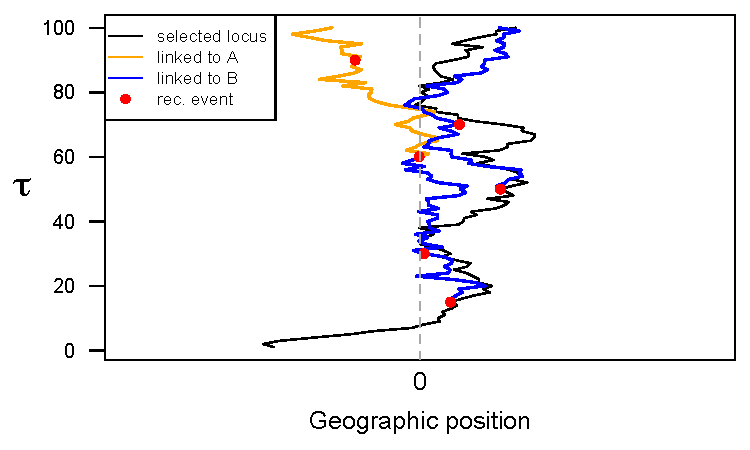
\includegraphics{figs/BM_schematic}
\caption{A cartoon representation of a haplotype under the model. The black line represents the path, backwards in time, of a site under selection ($L_B$) that is sampled in the present day. The center of the hybrid zone is defined at geographic position $x=0$, such that ancestry A segregates at lower frequency for $x>0$. Here, because of negative selection, $L_B$ migrates rapidly back to $x>0$ from a position $x<0$. Red dots represent recombination events along the entire haplotype. When a recombination separates two chunks of the sampled haplotype takes place, a branching event occurs and these splitting lineages are represented by colored lines (here the initial haplotype is broken up into 3 chunks over 100 generations). Subsequent recombination events can switch the selected background to which a chunk is linked.  Here, yellow lineages are linked to $L_A$ , and blue lineages are linked to $L_B$. Based on position 100 generations after contact, from right to left the chunks are of ancestry $(A,B,B)$.}\label{Fig:schematic}
\end{figure}

%As an approximation, we consider a cline of narrow width (look up cline width for underdominance, Barton/May?), such that the frequency of migrant alleles is exponential and negligible at distance away from the center of the hybrid zone. This means that recombination events that occur away from the center of the zone do not result in a change in $a$.


%%%%%%%% %%%%%%%%%%
\subsection*{Analysis}

In this section we aim to give both heuristics for how lineages move, 
that are helpful in establishing order-of-magnitude estimates,
and analytics, mostly in terms of partial differential equations needing numerical solution.

\paragraph{Establishment of the cline at the selected locus}
The deterministic theory predicts that after secondary contact,
the two alleles at the selected locus will form a stable cline \citep{Barton1979},
affecting neighboring loci as well.
First, we turn our attention to how the cline at the selected locus itself is formed.
Let $p(x,t)$ denote the frequency of the $A$ allele at spatial location $x$ and time $t$.  
Suppose that secondary contact occurred at time $t=0$, 
and that $p(x,0) = 1$ if $x<0$ and $p(x,0)=0$ if $x>0$.
% (In discrete computations, a deme at $x=0$ has $p(0,0)=1/2$.)
Let $\sigma^2$ be the mean squared distance between parent and offspring 
(i.e., the variance of the distribution of dispersal distance).
Assuming that: (i) alleles locally assort into diploids randomly, 
(ii) habitat and dispersal are homogeneous, and 
(iii) $s$ and $\sigma$ are small, then the commonly-used equation that $p$ solves is
\begin{align} \label{eqn:cline_pde}
    \dot p = \frac{\sigma^2}{2} \Delta p + s p (1-p) (2p-1) ,
\end{align}
where $\dot p(t,x)$ is the time derivative and $\Delta p$ is the Laplacian,
as derived in \citet{Bazykin1969}; for discussion of diploidy see \citep{christiansen1995genotypic}.
Although there is no known exact analytic solution to this equation, even in steady state, 
a good approximation to the equilibrium solution is that
$\lim_{t \to \infty} p(x,t) \approx (1+\tanh(-2x\sqrt{s}/\sigma))/2$ \citep{Bazykin1969}. 
This relies on numerous approximations, but the general conclusions should be quite robust: 
the stable cline has width of order $\sigma/\sqrt{s}$, and decays exponentially. 
Note that rescaling space and time by $\sigma/s$ and $1/s$ respectively in equation \eqref{eqn:cline_pde} results in a dimensionless equation,
implying that the cline establishes over a timescale of the order $1/s$. 
In other words, the cline is established through diffusion, which is slowed down somewhat by selection against heterozygotes. 
\alisa{I don't think I understand the independence from $\sigma$?}
\plr{It gets set up at speed $\sigma$ over a distance proportional to $\sigma$.}



\paragraph{Lineages at the selected locus}
Now suppose that the frequency profile of the selected allele $p(x,t)$ is known.
We will understand first how lineages of sampled individuals behave at the selected locus,
from which lineages at linked loci require only a minor modification.

Consider the collection of $A$ alleles found at geographic location $x$.
The expected number, among these alleles, that had a parent at location $y$ in the previous generation 
is proportional to the number of $A$ alleles that were at $y$ multiplied by the per-generation probability of dispersing from $y$ to $x$. 
In other words, lineages move as a random walk determined by the dispersal kernel,
but biased towards locations where the selected allele they carry is at higher frequency.
(Lineages are also biased towards regions with higher fecundity,
and thus away from the hybrid zone, but we assume that $s$ is small and ignore this.)

Making the same assumptions as for equation \eqref{eqn:cline_pde}, the derivation in Appendix \ref{apx:lineage_derivation} shows 
how the lineage of an $A$ allele moves as Brownian motion with speed $\sigma$
with drift $\sigma^2 \grad \log p(x,t)$ (i.e., it moves at speed $\sigma^2$ in the potential $-\log p$).
% \alisa{note to self to read through appendix when written}
To see why this is true, note that the probability that the parent of an $A$ allele found at $x$
lived at position $x+r$ is proportional to $\P\{R=r\} p(x+r)$, where $R$ is the random dispersal distance;
and so the mean displacement from offspring to parent is $\E[R p(x+R)]/\E[p(x+R)]$.
% $$ = \E[ R ( p(x) + R p'(x) ) ]/ p(x) + O(R^3) $$
Using that $\E[R]=0$ and $\E[R^2]=\sigma^2$
and expanding $p()$ to first order about $x$ shows that this mean displacement is approximately $\sigma^2 p'(x)/p(x)$,
\plr{Does that help at all?}

At a geographic position far from the center, $p=1$ to the left, and is proportional to  $\exp(-x\sqrt{s}/\sigma)$ to the right.
Therefore, roughly, lineages on ``their own'' side wander randomly,
while lineages on ``the wrong'' side are pushed at constant speed $\sigma/\sqrt{s}$ 
back towards the side where they are more common. 
\alisa{Is this a construction that we've enforced, or should this maybe go into the results section?}
\plr{This isn't a construction, it's a consequence of the model, so you're right, it is maybe a "result", but I think the explanation of why it happens belongs here.}
Since an $A$ allele must by definition have been inherited from the $A$ side of the barrier 
at the time of secondary contact, this push must get more intense the closer it is to the time of secondary contact.
Lineages of $B$ alleles do the same thing, of course, but in the opposite direction. 
% \alisa{I want to make a figure from the simulations that show the rapid retreat of wrong ancestries back to where they came from}

Note that this description gives more information than the steady-state solution,
since in that analysis only the ratio $\sigma/\sqrt{s}$ appears.
Here we see that lineages with $\sigma=10$ and $s=.16$ move quite differently
to lineages with $\sigma=1$ and $s=.0016$,
reflecting strong differences in selection against heterozygotes,
even though the stable clines have the same form.

\paragraph{Lineages at linked loci}
The behavior of a lineage at a linked locus is similar to a selected locus,
except that when in heterozygotes the lineage may move between backgrounds:
if we follow back through time a lineage at a locus we find linked to an $A$ allele, 
it will first tend to be inherited from ancestors to the left (as $A$ lineages drift to the left),
but if it spends time in the clinal region where recombination may happen,
it may be found to have been inherited from a $B$-carrying individual,
whose ancestors will tend to be more from the right.

Suppose we sample an allele today at a locus at recombination distance $r$ to the selected site.
We will follow its lineage back through time, using $\tau$ to denote ``time ago'' to avoid confusion.
If $X_\tau$ is the geographic location of its ancestor $\tau$ generations ago,
and $Z_\tau$ is the identity of the selected allele that ancestor carried,
then we say that $X$ moves as a diffusion pushed by either $\log(p)$ or $\log(1-p)$ (same as previously described movement of a selected allele),
and that $Z$ jumps between $A$ and $B$ at rate either $r (1-p)$  (from $A$ to $B$)or $r p$ (for $B$ to $A$).

We can describe this process formally in It\^o notation:
with $B_\tau$ a standard Brownian motion,
$T_B$ the first time $Z_\tau = B$, and likewise for $T_A$,
\begin{align}
    \begin{aligned} \label{eqn:lineage_motion}
        dX_\tau &= \begin{cases}
             \sigma^2 \grad \log(p(X_\tau,\tau)) d\tau + \sigma dB_\tau \qquad & \text{if } Z_\tau = A \\
             \sigma^2 \grad \log(1-p(X_\tau,\tau)) d\tau + \sigma dB_\tau \qquad & \text{if } Z_\tau = B 
        \end{cases} \\
        % \P\{ Z_{\tau+\epsilon} = B \given Z_\tau = A \} &= \epsilon r (1-p(X_\tau,\tau)) + O(\epsilon^2) \\
        % \P\{ Z_{\tau+\epsilon} = A \given Z_\tau = B \} &= \epsilon r p(X_\tau,\tau) + O(\epsilon^2)  .
        \P\{ T_B &> u \given Z_\tau = A \} = \exp\left( - r \int_0^u (1-p(X_s,s)) ds \right) \\
        \P\{ T_A &> u \given Z_\tau = B \} = \exp\left( - r \int_0^u p(X_s,s) ds \right) .
    \end{aligned}
\end{align}

\alisa{A conceptual cartoon of this process is shown in Figure~\ref{Fig:schematic}.}
\plr{Connect these up more.}



\paragraph{PDE for linked clines}
We can use this diffusion model for lineages to compute expected clines in ancestry,
i.e., the expected proportion of individuals who inherit from species $A$,
as a function of space, time, and position on the genome.
Precisely, we need the probability that 
an allele sampled $t$ generations after secondary contact at location $x$,
at recombination distance $r$ to a selected allele of type $z$,
is inherited from an individual of ancestry $A$,
where $z$ can be either $A$ or $B$.
We denote this probability $q_z(x,t,r)$.
In other words,
\begin{align}
    q_z(x,t,r) = \P^x \{Z_t = A\} .
\end{align}
(Recall that $Z$ depends implicitly on $r$.)
The description above implies that $q_z$ solves the following Kolmogorov backward equation:
\begin{align}
    \begin{aligned}  \label{eqn:q_pde}
    \dot q_A(x,t,r) 
            &= \sigma^2 \grad \log(p(x,t)) \cdot \grad q_A(x,t,r) 
                + \frac{\sigma^2}{2} \Delta q_A(x,t,r) 
            \\ &\qquad {} + 
                r (1-p(x,t))(q_B(x,t,r)-q_A(x,t,r))  \\
    \dot q_B(x,t,r) &= \sigma^2 \grad \log(1-p(x,t)) \cdot \grad q_B(x,t,r) 
            + \frac{\sigma^2}{2} \Delta q_B(x,t,r)
            \\ &\qquad {} + 
            r p(x,t) (q_A(x,t,r)-q_B(x,t,r))  ,
    \end{aligned} 
\end{align}
with boundary conditions $q_A(x,0,r)=1$ and $q_B(x,0,r)=0$, 
and where $\grad$ is the gradient, and $\Delta$ is the Laplacian.
\alisa{this is fwd-in-time notation. should we change it to bwd-in-time?}
\plr{This equation should be forwards in time, since it's the Kolmogorov backward equation
applied to a backwards-time process!}

We will have more use for the differential operators on the right-hand sides of these equations,
so define these as
$G^A = \sigma^2 \grad \log(p(x,t)) \cdot \grad + (\sigma^2/2) \Delta$
and
$G^B = \sigma^2 \grad \log(1-p(x,t)) \cdot \grad + (\sigma^2/2) \Delta$,
and then equation \eqref{eqn:q_pde} can be written more compactly as
\begin{align*}
    \dot q_A &= G^A q_A + r (1-p) (q_A-q_B) \\
    \dot q_B &= G^B q_B + r (1-p) (q_B-q_A) .
\end{align*}
In technical terms, $G^A$ and $G^B$ are the generators of the diffusions of $A$ and $B$ lineages, respectively.


\paragraph{Numerical computation}
To determine how the cline at a linked locus is expected to relax,
we can solve the partial differential equations \eqref{eqn:cline_pde} and \eqref{eqn:q_pde} numerically.
For instance, Figure \ref{fig:pde_clines} shows a heatmap of $p(x,t,r)$, 
the expected frequency of ancestry $A$ at location $x$ and time $t$ 
at a site at recombination distance $r$ from the selected site,
which is computed as $p(x,t,r) = p(x,t) q_A(x,t,r) + (1-p(x,t)) q_B(x,t,r)$. 
The equations are solved numerically in R, using the ReacTran package \citep{soetaert2012reactive}.

\paragraph{Haplotype lengths}
We can also find the probability of seeing an \emph{entire} block of genome (haplotype)
of a single ancestry at a given location and time.
To quantify haplotype abundances, we start by considering a segment of the genome between positions $a$ and $b$, relative to the selected site. 
We are interested in the probability $g_z(x,t;a,b)$ 
of finding an entire segment $(a,b)$ of ancestry $A$ in an individual having selected allele of type $z$,
sampled at spatial location $x$ at time $t$ after the cline has formed.

As in \citet{Sedghifar2015}, 
a given block of genome is inherited along a single lineage ever since the most recent recombination event
that fell within that block.
Prior to this, there are two lineages to follow (see Figure~\ref{Fig:schematic}),
and so lineages act like a particular class of labeled, branching diffusions,
where the total branching rate is conserved. 
We do not consider subsequent coalescence.
The general description of the process, again looking backwards in time, is as follows:
The lineage of a segment of genome moves as a linked locus described in equations \eqref{eqn:lineage_motion},
with recombination distance $r$ equal to the rate at which the segment recombines away from the selected site.
(If the selected site lies inside the segment, $r=0$.)
Additionally, at rate equal to the genetic length of the segment,
a recombination occurs, at which point the segment splits into two segments at a uniformly chosen location,
each of which proceeds as before, independently. 
Then, $g_z(x,T;a,b)$ is then the probability that all branches are found on the $A$ side of the hybrid zone
at the time of secondary contact $T$ units of time ago.

The resulting equation si similar to \eqref{eqn:q_pde} with a term added for branching,
which is written (omitting the $(x,t)$ for conciseness):
\begin{align}
    \begin{aligned} \label{eqn:g_pde}
        \dot g_A(a,b) 
        &= G^A g_A(a,b) + r(a,b) (1-p) (g_A(a,b)-g_B(a,b))
            \\ {} & \qquad 
            + (1-p) \int_a^0 \left(
                g_B(a,\theta) g_A(\theta,b)
                + g_A(a,\theta) g_B(\theta,b)
            \right) d\theta,
            \\ {} & \qquad 
            + p \int_a^b {
                g_A(a,\theta) g_A(\theta,b) 
            } d\theta
            - (b-a) g_A(a,b)  
    \end{aligned} ,
\end{align}
where $\theta$ is the genomic position of a recombination event, 
the integral $\int_a^0$ is zero if $a>0$ and likewise $\int_0^b$ is zero if $b<0$;
and $r(a,b)$ is the distance from the segment to the selected site:
$r(a,b)=0$ if $ab<0$ and $r(a,b)=\min(|a|,|b|)$ otherwise.
The equation for $g_B(x,t;a,b)$ is identical after exchanging $A \leftrightarrow B$ and
$p \leftrightarrow (1-p)$.
The boundary conditions are $g_A(x,0;a,b)=1$ and $g_B(x,0;a,b)=0$.

\paragraph{Numerical solutions}
Notice that equations \eqref{eqn:g_pde}
are hierarchical in $[a,b]$:
the equation for haplotype identity probabilities on a segment $[a,b]$ depends only on those probabilities for segments contained in $[a,b]$.
This allows for efficient numerical solutions,
described in more detail in Appendix \ref{apx:haplotype_calcs}.


\paragraph{Correlations in ancestry}
To compute correlations in local ancestry
(i.e., ``ancestry disequilibrium'', as in \citet{Pool2015,Schumer2016}),
we need only follow lineages at two sites, instead of an entire region,
the model described above requires only minor modifications,
and our numerical code can be used directly;
for more detail see Appendix~\ref{apx:haplotype_calcs}.


%%%%%%%% %%%%%%%%%%
\subsection*{Simulations}

We implemented forwards-time simulations of diploid individuals on a one-dimensional grid of demes
with non-overlapping generations and fixed population sizes (a Wright-Fisher model). Individuals are diploid, with haploid number $n=2$ chromosomes, each of length 1 Morgan. One chromosome pair harbors in its center (at position 0.5M) a single locus that reduces fitness by $s$ in heterozygotes, while the other contains no sites under direct selection.

Each deme has exactly $N_d$ diploid individuals at the start of each generation.
At the start of each generation, every individual migrates to a new deme  offset by $\lfloor Z + 1/2 \rfloor$ from their original position,
where $Z$ is a Gaussian random variable with mean zero and variance $\sigma^2$.
(The mean displacement is zero, and when comparing to theory we compute $\sigma$ as the standard deviation of this distribution.)
Migrants past either end of the range remain at the terminal demes.
Then, 
fitnesses are computed (heterozygotes at the selected locus have fitness $1-s$; homozygotes have fitness 1),
and in each deme $N_d$ pairs of parents are chosen, with replacement,
with probability proportional to their fitness and selfing allowed.
Since migration is not conservative, demes may have no available parents;
in this case, parents are chosen from other demes with probability proportional to fitness
multiplied by $\exp(-x^2/\sigma^2)$, where $x$ is the distance to the other deme.
The next generation is formed by carrying out meiosis in each parent
and combining the resulting gametes such that each pair of parents leaves one descendant.
Meiosis results in alternating blocks of the gamete's chromsome
being inherited from the two parental chromosomes,
with the blocks separated by a Poisson(1) number of uniformly chosen recombination points along the chromosome,
and the order of the parental chromosomes chosen randomly.
The simulation software works by recording for each chromosome
a list of ancestry breakpoints and the index of the ancestor in the first generation
that the chromosome inherited that region of genome from;
genotyping at individual loci was performed by looking up the ancestor's genotype.

Hybrid zones of varying ages were simulated under conditions of $\sigma=1$ and $s=0.1$ and $s=0.01$. From this we measure the length of unbroken tracts of ancestry $B$ surrounding a given position along a chromosome (if the locus in question was of ancestry $A$ the ancestry block had length $0$). These were compared to the output of neutral simulations with $s=0$
\plr{missing end of sentence?}

The simulations are executed in R, with scripts available on
\url{https://github.com/asedghifar/hybridzones}.

\begin{figure}
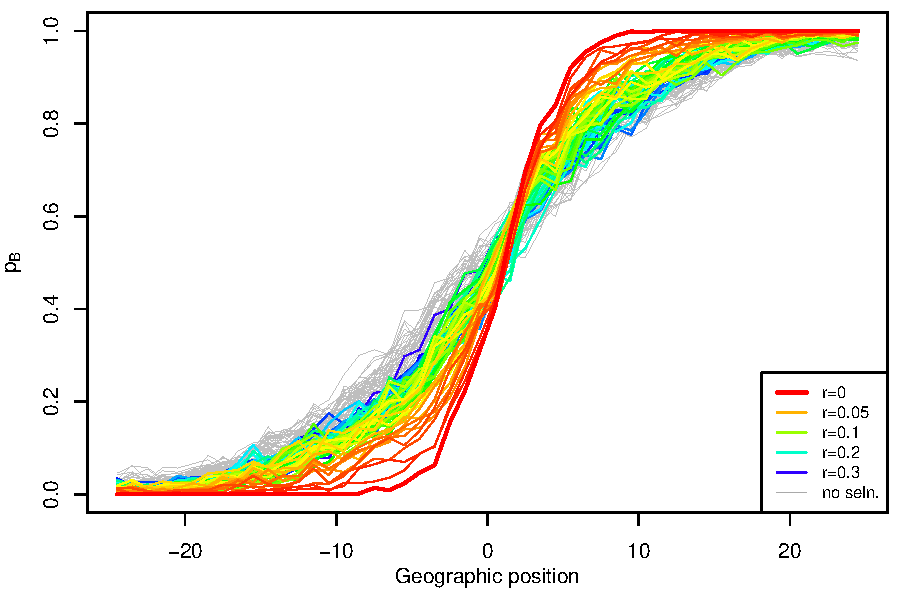
\includegraphics{figs/alleleFrequencies_sim}
\caption{
Frequency of ancestry B,
across geography and at several physical positions on the genome,
at $T=100$ generations after secondary contact. 
\plr{what is $s$?}
Each line represents a locus some distance $r$ away from the true target of selection, and $r=0$ represents the locus that is under selection. Grey lines represent the same positions from a simulation with
identical parameters except $s=0$.
    \plr{Add same figure for some different time points and maybe values of $s$ to the supplement.} 
}\label{alleleFreq_tau100}
\end{figure}

\subsection*{Measures of introgression}

\plr{This needs to be more precise, and should define and give a name to the ratio-of-adjacents statistic here, too.}

With the above theory and simulations, we are able to make predictions about patterns surrounding selected loci. In reality, however, such loci are not known, so it is useful to have per-site statistics that may allow for detection of candidate targets of selection. The most straightforward measure is $l_I(m)$ the length of haplotype chunk that a sampled chunk containing genomic position $b$, conditioned on ancestry $I$ at the site. Based on our expectation of the distribution of block lengths, we compute $l_B(m)$ for $m$ across a chromosome. 

Another statistic is the cumulative probability $C_I(m)$ of a sampled chunk encompassing position $m$ being longer than a chunk sampled from the distribution of all chunk lengths across the genome in the population. 

Additionally, we look at the mean value of these statistics in the two chunks, $m-$ and $m+$, that flank the block of unbroken ancestry containing $m$.











%\subsection*{Data}
%We compare the predictions of our model to genomic data obtained from individuals sampled a naturally occurring hybrid zone between \emph{Mus m. musculus/M. m. domesticus} \cite{Turner2011,Turner2014}. The genomic data generated by \citep{Turner2014} was for a mapping population generated by mating wild-caught individuals. Because some individuals were mated multiple times, the mapping population comprises many closely related individuals. We approximate wild population samples by restricting our analysis to genotyped individuals that had both parents sampled in the same location in such a way that none of the individuals shared a parent (see table for list of individuals). Approximately 280,000 SNPs were represented in the final dataset. 

%Ancestry blocks were estimated using ChromopainterV2 \cite{Lawson2012} and STRUCTUREv2 \cite{Falush2003} with $k=2$.


%Although we expect the age of this hybrid zone to correspond to historical human movement, and therefore be thousands of years old \cite{Teschke2008}, weighted the physical scale of ancestry-disequilibrium (both in the form of weighted ancestry-LD \citep{Loh2013} and ancestral block lengths) suggest relatively recent hybridization. Specifically, the high LD between quite distantly linked SNPs in the FS population suggests that a relatively high proportion of early-generation hybrids, whereas the rapid decay of LD in the the TU population reflects a much older hybridization event. Importance of geographic distribution of popgen patterns. 

%\begin{table}
%\begin{tabular}{l|c|c}
%Individual ID  & Population \citep{Turner2011} & Longitude(E)\\
%\citep{Turner2014}& \citep{Turner2011}&\\
%\hline
%FP112 & FS&11.665\\
%FP67 & FS &11.665\\
%FP114 & FS &11.665\\
%FP79 & FS &11.665\\
%FP152 &  FS &11.665\\
%FP11 & GL &11.965\\
%FP111&GL &11.965\\
%FP59 & HA  &11.721\\
%FP92 & HA &11.721\\
%FP7 &  HA  & 11.721\\
%FP45 & HA&11.721\\
%FP244& HO &11.693\\
%FP9&   RE&11.994\\
%FP5 &  RF&11.767\\
%FP78 &  SO &11.539\\
%FP52 &  SO &11.539\\
%FP180& SO &11.539\\
%FP14 & ST&11.539\\
%FP40 & ST&11.539\\
%FP145 & TU&11.748\\
%FP29&  TU&11.748\\
%FP135& TU&11.748\\
%\end{tabular}
%\end{table}

\section*{Results}

\section*{Single-locus behavior}

From previous results, we expect that far away from the zone center, variants under negative selection will be rare \citep[for demonstration of this theoretical result, see e.g.][]{May1975,Slatkin1973,Barton??}, and correspondingly, clines at closely linked sites are narrower.
This is seen, for instance, in Figure~\ref{alleleFreq_tau100}. 

\plr{When discussing haplotype lengths, say what happens at different $s$ and $T$.}

\paragraph{The timescale over which linked clines relax:}
Although loci not under selection can in principle spread across the cline unimpeded,
in practice it can take quite some time for even unlinked neutral loci to homogenize,
due to the decreased fitness of heterozygotes \citep{Barton1986}
and the relative slowness of diffusive movement \citep{Sedghifar2015}.
We are interested, for samples across a cline $T$ units of time after secondary contact, how far away from the selected locus one has to look to see clines that resemble the genome-wide mean.


A linked cline will begin to flatten out if there is an appreciable chance that a lineage at the linked locus initially coupled with an $A$ allele 
at some point recombined from an individual carrying the $B$ allele.
This implies that loci closer than $1/T$ to the selected site will not have a substantially wider cline than the selected cline.

In principle, the genomic window about the selected site
in which clines remain narrow could be quite a bit wider,
since the only way to move linked lineages between selected backgrounds is via recombination in a heterozygote,
and heterozygotes for the selected allele are only found at high frequency in the cline.
The majority of lineages are generally pushed away from the cline but have no bias far away,
so the amount of time a lineage spends in heterozygotes should grow as $\sqrt{T}$ for large $T$,
and so the width of the genomic region showing clines about the selected locus could be 
substantially larger than $1/T$. However, this distinction appears hard to observe for realistic parameter values.



\plr{Figure showing this? 
    For instance, either: (a) time-genome heatmap of number of heterozygotes (from PDE);
    or (b) a few time-space heatmaps of frequencies at different values of r (from PDE);
    or (c) a few space-genome heatmaps of frequencies at different times (from sims)
}



%%%%% %%%%%%%%%%
\subsection*{The distribution of ancestry tract lengths}

The distribution of contiguous ancestry block lengths necessarily contains more information than allele frequency alone. We are interested specifically in the how tracts of ancestry surrounding the selected locus compares to the rest of the genome. 
The raw data -- ancestry assignments for a few individuals sampled from across space --
is shown in Figure~\ref{Fig:resistanceToIntrogression1000g},
showing distinct patterns across geography and the genome.

As expected, regions surrounding a locus under selection are more resistant to introgression,
as seen in figures~\ref{Fig:resistanceToIntrogression1000g} and \ref{Fig:resistanceToIntrogression100g}).
When present, however, we expect haplotypes including the locally less common allele
to be longer than the genome-wide average.
Indeed,
as shown in Figures \ref{Fig:blockLengths} and \ref{Supp:blockLengthHeatmap},
the mean length of such haplotype blocks are up to three times longer
than the average for that geographic location.
\plr{Write down in the section on statistics what exactly you normalize by:
is it the mean for that geographic location?  Or, what?}
% This pattern provides a potential avenue for identifying targets of selection by looking for a signal of increased $l_B$ or $l_A$ for positions surrounding a selected site, compared to the genome-wide background  at geographic sites far from the center of the zone (Figure~\ref{Fig:blockLengths},~\ref{Supp:blockLengthHeatmap}). 
The mean haplotype length found without conditioning on ancestry ($l_\cdot$)
also shows an small increase near the selected locus,
but it is much smaller (see Figures \ref{Supp:blockLengthHeatmapNoAnc} and \ref{Supp:blockLengthNoAnc}).

We expect that, in the absence of selection, blocks of $A$ ancestry across the genome 
will tend to be shorter the further one goes into the $B$ side of the cline,
because they have had more opportunities to recombine with $B$ haplotypes. 
However, we expect that stretches of $A$ ancestry containing a selected site will be longer
than those that do not contain the selected site at the same spatial location,
because lineages containing the selected site have usually been inherited from the $A$ side of the cline recently. 
As discussed above, we expect these lineages move at speed roughly $\sigma/\sqrt{s}$,
so (selected) $A$ alleles at distance $x$ from the cline center
to have last had an ancestor on the $A$ side of the cline around $x \sqrt{s}/\sigma$ generations ago 
(compared to $x^2/\sigma^2$ for a neutral allele),
and so the enclosing $A$ haplotype is no longer than $\sigma/(x \sqrt{s})$.
\plr{(check predicted decay of mean length $1/x$ in simulations?)}
For linked haplotypes not containing the selected site, the situation is more complicated, and harder to intuit.


%%%%%%
\begin{figure}
    \begin{center}
    \end{center}
    \caption{
        \textbf{Haplotype length distributions},
        comparing numerical solutions to simulations.
        At one time, plot 
        probability of seeing a haplotype of length at least $r$ covering that position on the genome,
        against (a) position on the genome, at a few spatial locations;
        or (b) spatial location, at a few positions on the genome.
        \plr{maybe?}
        \label{fig:haplotype_lengths}
    }
\end{figure}




\subsection*{Lengths of adjacent blocks}

\plr{Define this statistic and put in the Summary Stats section. Also, move this up with the haplotype length stuff?}
We find that $l_A(k\pm)$, the length of blocks adjacent to blocks containing $k$, are shorter than average when $k$ is in a block of unbroken ancestry surrounding a selected site on the ``wrong side'' of the side of the zone.  (Figure~\ref{Supp:adjacentBlocks}). This pattern provides an avenue for further enhancement of the block-length signal around a selected locus, by taking the ratio $\frac{2\sum{l_B(k_i)}}{\sum{l_A(k_i+)+l_A(k_i-)}}$ of mean block lengths surrounding a site with the mean length of adjacent blocks (Figures~\ref{Supp:ratioBlockAdjacent},~\ref{Supp:ratioBlockAdjacentHeatmap}).

%This pattern means that we can further refine the signal of block lengths around a selected locus, by measuring the ratio $\frac{2\sum{l_B(m_i)}}{\sum{l_A(m_i+)+l_A(m_i-)}}$ of mean block lengths surrounding a site with the mean length of adjacent blocks (Figures~\ref{Supp:ratioBlockAdjacent},~\ref{Supp:ratioBlockAdjacentHeatmap})



%We are interested specifically in the distribution of the length of continuous tracts of ancestry surrounding the selected locus. Far away from the zone center variants under negative selection will be rare \citep[for demonstration of this theoretical result, see e.g.][]{May1975,Slatkin1973,Barton??}, however, when present an unfit migrant haplotype is expected to be longer than a neutral migrant haplotype. Figure X shows the estimated probability density (pdf), of unbroken tract of ancestry B surrounding the selected locus, conditioning on a haplotype being of ancestry B at the selected locus. Compared to the expected density of tract lengths surrounding neutral loci, tracts of ancestry B around the selected locus are longer.

%Of particular interest is whether or targets of selection could potentially be identified by a signal of larger ancestry tracts surrounding them compared to a genome-wide background. To demonstrate this, we simulated a chromosome of length 1M with a selected site at position 0.5M. For a set of positions $\mathbf{m}$ along the chromosome, we computed the length $l_B(m_i)$ of the surrounding unbroken block of ancestry. There is a detectable signal of increased block length surrounding selected loci when conditioning on the less-fit ancestry (Figure~\ref{Fig:blockLengths},~\ref{Supp:blockLengthHeatmap}) at geographic sites far from the center of the zone. A signal is also present for, but less well resolved when ancestry is not taken into account (Figures~\ref{Supp:blockLengthHeatmapNoAnc},~\ref{Supp:blockLengthNoAnc}).



\begin{figure}
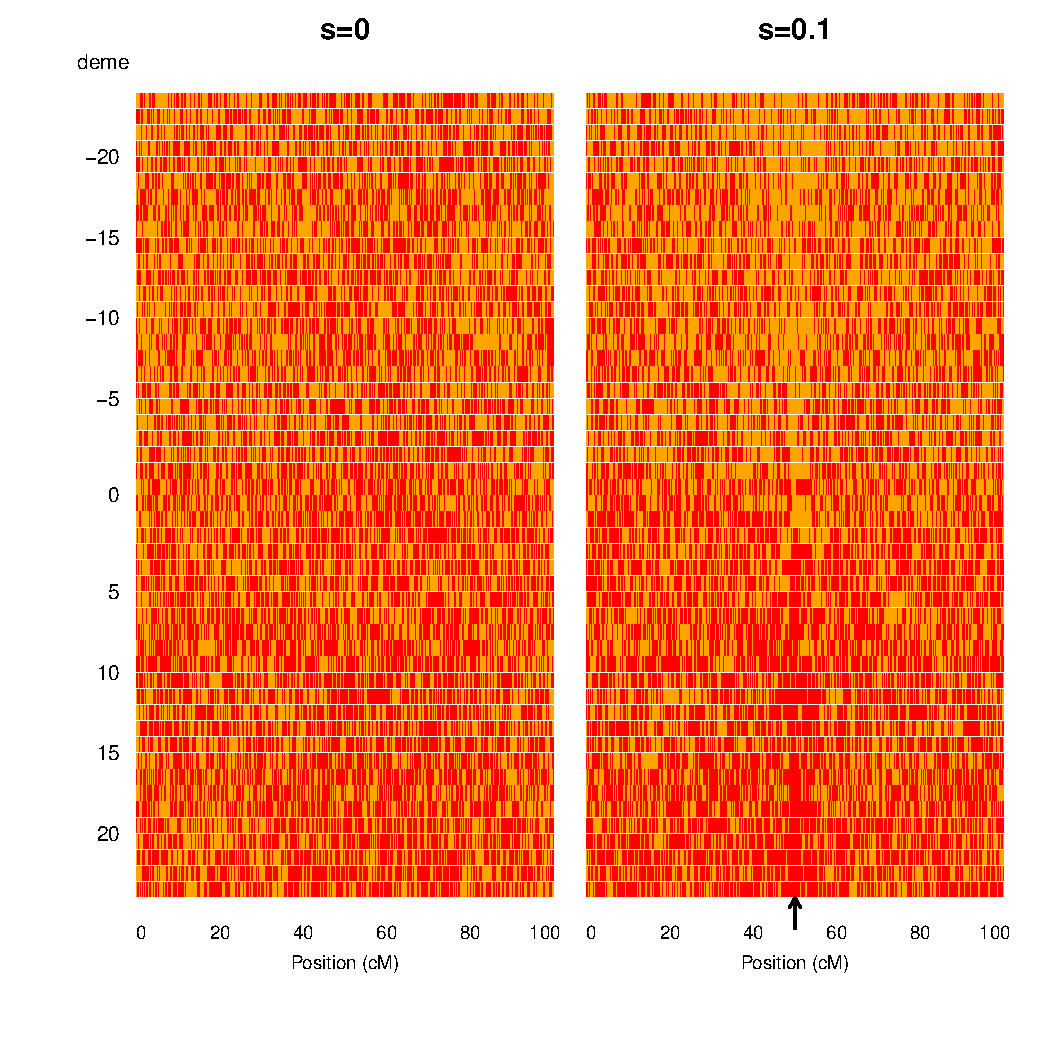
\includegraphics[width=\textwidth]{figs/plot_chromosomes_tau1000}
\caption{Randomly sampled chromosomes  across a hybrid zone of age $T=1000$. Here we compare chromosomes of length 1M from a neutral zone to one that has a single under-dominant locus ($s=0.1$) in the middle of the chromosome (indicated by black arrow). Red blocks along the chromosome denote ancestry $B$, and orange blocks are ancestry $A$. Regions surrounding the selected site are failing to introgress.
    \plr{Add same figure for some different time points and maybe values of $s$ to the supplement.} 
}\label{Fig:resistanceToIntrogression1000g}
\end{figure}

\begin{figure}
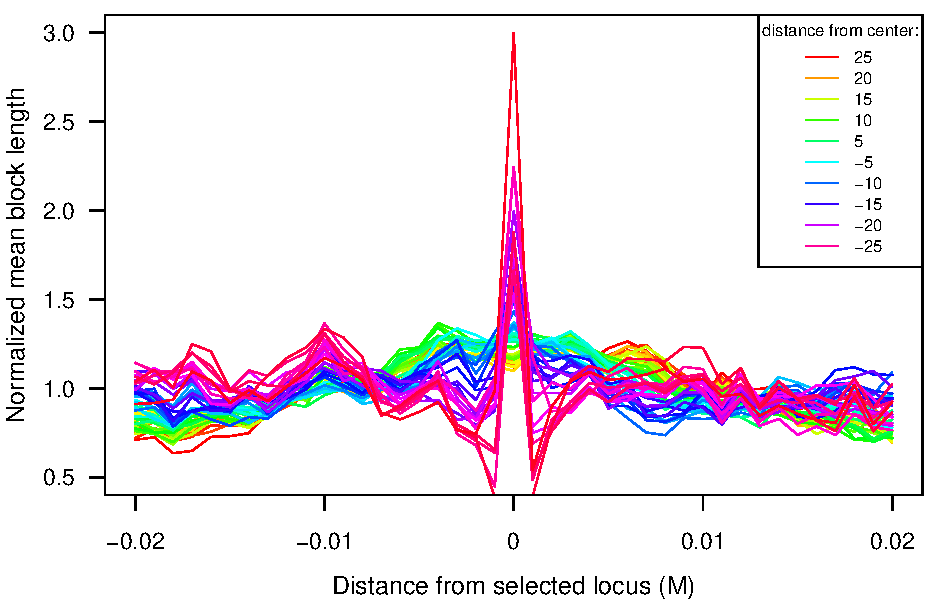
\includegraphics{figs/blocksAlongChromAncBConditioning}
\caption{Mean block length, $l_B(k_i)$, along a simulated chromosome of length $1M$ with selected locus at position $0.5M$. Here each line represents  $l_B(\mathbf{k})$, the mean block lengths in a given deme, and is normalized by mean block length $l_B(k_i)$ along the chromosome in the deme.
    \plr{what is $T$ and $s$? also, add version with different $T$ and/or $s$ to the supplement.}
}\label{Fig:blockLengths}
\end{figure}


\subsection*{The number of `unfit' ancestors}

\plr{This needs a bit more precise discussion.}

Although our analytical model does not account for coalescence, we are able to partially trace the genealogy of haplotypes in our simulations. In particular, we wish to know the relative number of ancestors from $T$ generations ago that are represented in present day populations at a given locus, given the frequency of a particular ancestry. This is a reflection of the average size of a haplotype family. We find that, as distance from the zone center increases, the average family size of an ancestor from time $T$ decreases (Figure~\ref{Fig:family_size}). One interpretation of this observation is that migrants tend to leave few offspring before being removed from the population by selection. This can potentially provide additional signal for characterizing lineages strongly influenced by selection.

\begin{figure}
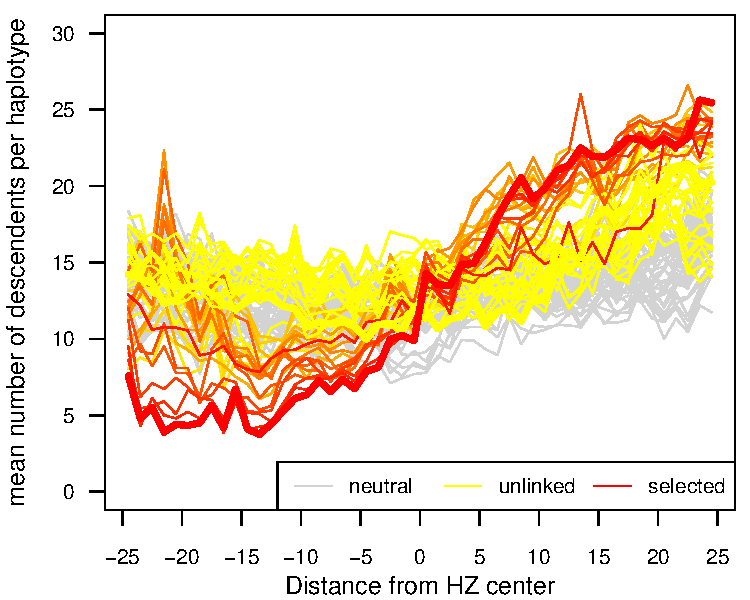
\includegraphics{figs/number_of_ancestors_tau1000}
\caption{The number of individuals of ancestry B per number of ancestors from secondary contact occurring $T=1000$ generations ago, represented across geographic space. Each red or orange line represents a site some distance away (ranging from 0 - 0.01) from the selected site (here $s=0.01$ and $\sigma=1$). Yellow lines are corresponding positions on an unlinked chromosome with no selected loci, and grey lines are corresponding positions in a simulation with no selection.  Bold lines depict the target of selection when present, and corresponding position on chromosomes not harboring any selected sites.}\label{Fig:family_size}
\end{figure}


\section*{Discussion}

%\plr{This first paragraph sounds like the Introduction.  A brief recap here is good: maybe something like:
%    Our goal in this paper was to describe cline formation and haplotype structure around a new hybrid zone,
%   which we have done using both theory and simulation.
%   Our most useful observations are that clines establish over time $1/s$,
%    and that lineages of selected loci found on the side of the hybrid zone where they are at a disadvantage
%    tend to move back towards the side where they are common
%   at speed $\sigma/\sqrt{s}$.
%   This predicts that blocks of ancestry are longer near the center, flanked by shorter ones ...
%}

\alisa{Using a combination of theory and simulations, we present a description of the process of cline formation and haplotype structure in a relatively young (i.e. non-equilibrium) hybrid zone.
We show that clines establish over time $1/s$, and that lineages of selected loci tend to move back towards their `ancestral home' when in a geographic region where they  are unfit. 
This occurs at speed $\sigma/\sqrt{s}$. Based on this we predict, and observe in simulations, that blocks of ancestry surrounding these selected loci are longer, especially when distant from the center of the cline. 
This extends previous theoretical work on hybrid zones, which has primarily focused on stable clines in allele frequency and  suggests approaches to interpreting patterns of variation in hybrid zone populations, as well as detecting targets of purifying selection in hybrid zones.}

\alisa{\paragraph{Targets of selection}}
Most attempts to identify loci under selection in hybrid zones identify alleles that are exceptional in terms of frequency across space, or genome-wide admixture proportion \citep{Porter1997,Gompert2012}.  
Current genomic approaches can provide an additional rich source of information when applied to the study of hybrid zones. In particular, ancestry deconvolution facilitated by programs such as  hapMIX \citep{Price2009}, LAMP \citep{Sankararaman2008} and fineSTRUCTURE \citep{Lawson2012} provides researchers with a measure of the length of ancestry tracts across the genome and this information has been used extensively to infer the demographic history of hybridization/admixture \citep[e.g. ][]{Hellenthal2014,Schumer2014}. In order to interpret these patterns in the context of a hybrid zone, we set out to understand the impact of selection on patterns of ancestry tract lengths, and here present an expectation of block-length patterns throughout a hybrid zone. Importantly, we find that selection against hybrid incompatibilities leaves a distinct genomic signature in the form of long contiguous blocks of ancestry around these loci.


%However, how selection influences the length of tracts of ancestry around selected sites in hybrid zones has received much less attention. We we present an expectation of ancestry block lengths in hybrid zone. We find that selection against hybrid incompatibilities leaves a distinct genomic signature in the form of long contiguous blocks of ancestry around these loci.   

\plr{(selected lineages drift back, so haplotypes are longer)}
Our finding that long blocks of ancestry surround selected sites in hybrid zones reflects the intuition that regions surrounding selected loci are going to \alisa{introgress less readily?} have a harder time introgressing. 
Thus we can interpret this pattern as Brownian motion with drift in which an ancestry which finds itself on the wrong side of a hybrid zone rapidly moves, backwards in time, across space to the ``correct'' side of the hybrid zone.  In other words, selected alleles that have, by chance, encroached deep into the other side of the hybrid zone have likely done so quite recently, as they cannot survive long in such hostile territory.  
\alisa{As a result, the haplotype that the selected locus resides on has few opportunities for recombination on the `wrong' side, which is reflected in long blocks of contiguous ancestry.}
%The recently of this movement results in few opportunities for recombination and is therefore reflected in long blocks of contiguous ancestry.  
\plr{This next stuff is said later, under "Assumptions"; maybe should be moved there.}
\yb{While our theory focusses on a spatially arranged hybrid zone, it is likely that our results extend to alternative models of hybridization including models of assortative mating and hybrid swarms. This is because regardless of the specific demographic model, selection against hybrids will severely limit opportunities for recombination between ancestries around incompatibilities.}

\subsection*{Additional signatures around selected loci} 

\plr{(selection increases drift and migrant families are small; need better words/description here.)}
We further found that the long blocks of ancestry around selected sites on the wrong side of the hybrid zone will likely come from a relatively large number of independent ancestors per individual of that ancestry. (Figure~\ref{Fig:family_size}). % is this right 
This result also reflects the fact that, on average, haplotypes on the ``wrong'' side of the hybrid zone tend to be recent migrants and have therefore had few descendants. 

\plr{(long blocks adjacent to short ones: combine with bit on long blocks)}
In addition to our finding that ancestry surrounding selected sites is relatively long, our simulations revealed a consistent and unexpected finding. We found, on a given side of the hybrid zone, a transition from the locally adaptive ancestry at the selected site to the alternative ancestry at a closely linked site was short-lived (Figure~\ref{Supp:adjacentBlocks}). Put differently, blocks of `wrong' ancestry that do not overlap the selected site but are closely linked are exceptionally short. A simple intuitive explanation for this pattern suggests itself - loci physically linked to the selected sites can only survive on the wrong side of the hybrid zone for a reasonable amount of time if they recombine away from their ancestry at the locally adaptive site. Because it is then tightly linked to the alternate ancestry at the selected site, this ancestry chunk will largely recombine with the alternate ancestry, and therefore decay rapidly. \yb{This finding suggests that, despite the fact that haplotypes surrounding incompatibilities might be quite long, genome scans may have the power to extract fine-grained regions near selected loci from the large chunks of ancestry that will often flank these regions.}

\plr{(we'll be able to see this soon)}
These two novel findings may be beyond detection in current research programs that often make use of low-density genetic markers for which phase is unknown. However, as the const of sequencing continue to drop and long-phased reads become more common, access to data pertaining to these observations could further aid in identifying selected sites in hybrid zones.  %\yb{(CITE doi:10.1038/nbt0515-433 )} %Startups use short-read data to expand long-read sequencing market Michael Eisenstein Nature Biotechnology 33, 433?435 (2015) doi:10.1038/nbt0515-433 Published online 12 May 2015
\alisa{In the meantime, patterns of elevated pairwise LD, which is more easily computed from readily available data, surrounding selected loci could offer an approximation to these findings.}

\subsection*{Paths to inference}

\plr{(combine with haplotype length stuff above)}
Our results suggest that a few natural statistical summaries could help identify selected loci in hybrid zones. 
Specifically, the statistic $l_z(k)$ -- the genetic length of ancestry surrounding a site of a given lineage -- and similarly,  and similarly $l_z(k\pm)$, could provide a simple and informative summary. 
This statistic, perhaps in relation to the length of ancestry around adjacent sites, could be developed into an approach to scan genomes from hybrid zones to identify putatively selected loci. 

\subsection*{Assumptions}

\plr{(het. disadvantage)}
We made numerous simplifying assumptions to derive our analytical and also in the execution of the simulations. %Thus before our results can be profitably used for inference, it is worthwhile to  reflect on our assumptions and their consequences. 
Foremost, we have assumed that selection acts against heterozygotes, and that there is a single underdominant locus. This situation is uncommon in nature, since underdominant loci cannot invade when rare, and thus this assumption is likely rarely met. \alisa{We believe, however, that this assumption is unlikely to drastically influence our results, and previous results demonstrating that underdominant loci share similar properties as more realistic genetic models such as ecological selection, mean that our findings here are somewhat generalizable} \citep{Barton1989, Barton1993}

\plr{(one locus only)}
The assumption about the density of selected loci, however, may have greater consequences. Our model, which focuses on a single selected site is likely to be still relevant to cases in which there are only a small number of selected loci scattered throughout the genome. However, our predictions may differ significantly from scenarios in which the density of selected sites is high. Specifically, numerous selected sites within one ancestry block would likely act to both  increase the strength of selection, and to generate a longer unit which cannot be effectively broken up by recombination   \citep{Barton1983,Kruuk1999}. Such regions would likely be surrounded by even greater chunks of unbroken ancestry -- a result reflecting  greater $s$ and relatively short map distance between linked incompatibilities -- \alisa{and will impact expectations of genome-wide patterns of clines and block lengths. In terms of detecting targets of selection, such sites will be a common limitation among many approaches to identifying selection.}

\plr{(1D)}
For ease of calculations, our analytic model assumes a continuous and smooth one-dimensional spatial structure of the geographic landscape. This allows us to derive analytic expressions that track lineages, and is an example of the more general idea of duality for particle systems \alisa{I think this may be beyond the average ME reader?}. 
\plr{Tracking lineages is duality, has nothing to do with 1D, though.}
However, this assumes a large population density limit that excludes \plr{coalescence} and makes linages Markov \alisa{not sure about what point this is making? Is there a better way to state this for our intended audience?}.  
\plr{It means we're ignoring drift/coalescence, an important source of stochasticity; but that's the next paragraph too}
In contrast, our simulations model regularly spaced demes. In reality, populations may be patchily connected, especially at the edges of species ranges where hybrid zones may occur. While we still believe that the genomic signature of long ancestry chunks around selected sites will still hold in these situations, the strength of this expectation is unclear.

Lastly, the analytic model presented here lacks \yb{both coalescence and a true pedigree structure}. \alisa{This can result in an underestimate of covariance in ancestry, as we have ignored sharing through genealogy \cite{Liang2014}.} 
The broad agreement between our analytic predictions and simulations that include an explicit pedigree structure suggests that this assumption does not have a severe qualitative impact on our major results, especially for all but the most recently formed hybrid zones.


%One major assumption of our model is that selection acts against heterozygotes --i.e. that loci are underdominant. 
%Under dominance is quite rare in nature, because underdominant loci cannot invade when rare, and thus our major assumption is likely rarely met. 
%We believe, however, that this assumption is unlikely to drastically influence our results --- previous research has found that under dominant loci  have similar proprrties in hybrid zones as more realistic genetic models, such as ecological selection \yb{(CITE: (BARTON and HEWITT 1989; BARTON and GALE 1993)}. 
%An additional assumption of our analytical model is that we ignore coalescence.  
%The broad agreement between our analytical and theoretical results suggests that this assumption will also have negligible effect on our results. 

%Also, parent-offspring dispersal is not the same thing as successful-offspring-parent dispersal.


%\alisa{epistasis}
%\alisa{selection here is STRONG, not sure how well this will work on systems in which selection on any given locus is small (most systems)}


\subsection*{Islands of divergence}  

\plr{seems like a nice point but should be more positive and less snarky.  "Thanks to studies like these, it is time to start explicit modeling, as we have done here..."}
The past years have witnessed evocative metaphors of seascapes to describe heterogeneous patterns of genetic divergence across the genome.  
The metaphors of ``islands'', ``continents'' and ``archipelagoes'' of divergence \citep{Turner2005, Nosil2009} have inspired much research (and controversy  \citep{Noor2009,Cruickshank2014}) in speciation genomics, but have been largely descriptive.  
REFS  http://www.ncbi.nlm.nih.gov/pubmed/16076241 http://www.ncbi.nlm.nih.gov/pubmed/19143936 http://www.ncbi.nlm.nih.gov/pmc/articles/PMC2809014/ http://onlinelibrary.wiley.com/doi/10.1111/mec.12796/abstract
We hope that our work provides a path towards thinking about the process of heterogeneous divergence more concretely. % in terms of the processes of migration, and selection influencing patterns of ancestry across the genome of hybridizing populations.
Specifically, we provide a natural interpretation of large contiguous chunks of ancestry, as sites linked to those experiencing selection.   
Overall, focusing on lengths of ancestry blocks across the genome brings focus to the processes of migration and selection rather than high-level summaries that are somewhat abstracted from the evolutionary process. 


\subsection*{Future directions}

\plr{Perhaps delete this paragraph? A small note saying should check power with simulations up where we discuss the statistic would do.}
Our work has highlighted distinct genomic signatures accompanying hybrid incompatibilities. 
We suggest that such signatures could be combined in an inference framework that aims to identify incompatibilities from genome scans of hybrid zones.  
However, doing so requires careful evaluation of potential signals of an incompatibility. 
For example, should we consider jointly lengths of ancestry and allele frequencies to identify incompatibilities?
Will dividing haplotype length by the length of adjacent haplotypes add power to tests because of the extra information contained in this measure, or add noise because of chance variation in these statistics.  
Validation of the effectiveness of our proposed statistics, especially under demographic models that differ from the one dimensional hybrid zone explored above, will  provide a guide on how our results can be used to learn about selection from the distribution of ancestry tract lengths. We note, however, that power to detect regions under selection will depend on a number of parameters, such as $s$ and $T$

\plr{Remove "Future directions", title this "The hybrid filter", and discuss the hybrid filter ideas we had?}
Throughout, we have focussed on hybrid incompatibilities, however, the possibility that some loci adaptively introgress across hybrid zones has excited many biologists \citep{Arnold2004}.   
The best characterized example of adaptive introgression comes from the vitamin K epoxide reductase subcomponent 1 (vkorc1), which seems to have spread from Algerian mice \emph{Mus spretus} to house mice \emph{Mus musculus} from because it confers resistance to the anticoagulant rodenticide, warfarin. \citep{Song2011}. 
Future work could dress expected genomic signatures of adaptive introgression in hybridizing populations using the number and length of haplotypes of non-native ancestry. 
Doing so requires an understanding of how positive selection shapes ancestry block lengths in these cases. 



\subsection*{Theory and simulation}
In this work, we have taken two complementary approaches,
using both simulation and theory, and comparing the two.
As usual, simulations make fewer biological simplifications,
while theory provides more generalizable conclusions.
To do this, we have described the branching diffusion process that approximates
the lineages along which haplotypes are inherited.
Since the expected motion of a lineage depends on the local frequencies of the selected alleles,
these diffusions are time-inhomogeneous.

The diffusion model for lineages predicts that quantities of interest solve sets of coupled partial differential equations (PDE),
which we have written down.
As there are no known analytical solutions to these PDE,
we have constructed numerical solutions (and provide the source code for doing this).
A main role of these solutions in our work has been to verify that theory based on the diffusion model of lineages
matches the simulations.
These solutions easily and quickly provide predictions of joint frequencies at small numbers of loci.
However, due to the high dimensionality of the haplotype problem (spatial position $\times$ time $\times$ endpoints of the haplotype),
numerical solutions for mean haplotype lengths along the genome can be as computationally intensive as simulations
(although are substantially less noisy).
More work could be done to develop more efficient methods of solution,
but it may be better to perform more biologically realistic forwards-time simulations that includes coalescence and drift.
Nonetheless, the PDE approach is easily modified to provide predictions for spatial and temporally inhomogeneous systems --
for instance, across maps of real landscapes.


\subsection*{Simulation and analysis code}

These are written primarily in R, and are available HERE.

\bibliographystyle{molecularEcology}
\bibliography{library,references}

\appendix
\setcounter{table}{0}
\renewcommand{\thetable}{S\arabic{table}}
\setcounter{figure}{0}
\renewcommand{\thefigure}{S\arabic{figure}}


\section{Rescaling a discrete model to obtain the lineage motion}
\label{apx:lineage_derivation}

For concreteness, here we describe a discrete model that rescales to the continuous model we consider.

In this discrete model, the total number of individuals at location $x$ is $N(x)$,
and we count ``individuals'' as \emph{haploid},
so each individual is of type either A or B at the selected locus,
and the proportion of individuals of type A and location $x$ and time $t$ is $p(x,t)$
(but, we often neglect the $t$).
Suppose that type A individuals at location $x$ reproduce at rate $s_A(x)$, 
and likewise type B at rate $s_B(x)$.
Assuming locally random mating, we will then have that
$s_A(x) = 1 - s (1-p(x))$ and $s_B(x) = 1 - s p(x)$.

At reproduction, individuals recombine with others in the same location,
with recombination occuring between the locus we follow and the selected locus with probability $r$,
and the offspring choose a new location $y$ with probability $m(x,y)$.
The population dynamics are random, 
but suppose that $N(x)$ is sufficiently large that these do not vary substantially with time.
Suppose this is a Moran model.
There are four things that can happen:
\begin{enumerate}
    \item[$x\xrightarrow{AA}y$] One type A individual at location $x$ reproduces, 
        either does not recombine or recombines with another type A,
        and sends the offspring to $y$.
    \item[$x\xrightarrow{AB}y$] An individual at location $x$ reproduces, 
        recombines with the other type,
        and sends to $y$ an offspring
        who inherits at the selected locus from the type $B$ parent 
        and the at the neutral locus from the type A parent.
    \item[$x\xrightarrow{BA}y$] An individual at location $x$ reproduces, 
        recombines with the other type,
        and sends to $y$ an offspring
        who inherits at the selected locus from the type A parent 
        and the at the neutral locus from the type $B$ parent.
    \item[$x\xrightarrow{BB}y$] One type $B$ individual at location $x$ reproduces, 
        either does not recombine or recombines with another type $B$,
        and sends the offspring to $y$.
\end{enumerate}
These four things happen at rates:
\begin{align}
    & x\xrightarrow{AA}y & \qquad w_{AA}(x,y) &= p(x) s_A(x) \left(1 - r (1-p(x)) \right)  N(x) m(x,y) \\
    & x\xrightarrow{AB}y & \qquad w_{AB}(x,y) &= r p(x) (1-p(x)) \frac{s_A(x)+s_B(x)}{2} N(x) m(x,y) \\
    & x\xrightarrow{BA}y & \qquad w_{BA}(x,y) &= r p(x) (1-p(x)) \frac{s_A(x)+s_B(x)}{2} N(x) m(x,y) \\
    & x\xrightarrow{BB}y & \qquad w_{BB}(x,y) &= (1-p(x)) s_B(x) \left(1 - r p(x) \right) N(x) m(x,y) 
\end{align}

Note that at equilibrium, we require $N$ to solve
\begin{align}
  0 = \sum_y N(y) m(y,x) \left\{ p(y)s_A(y)(1-p(x)) - (1-p(y))s_B(y)p(x) \right\} .
\end{align}

\subsection*{Lineage movement}

These rates tell us the rates at which a lineage will move, backwards in time.
For instance, the rate at which a lineage at the selected locus
currently in a type A individual at location $x$
jumps to another type A individual at location $y$ is equal to the rate of influx of migrants from $y$
divided by the number of A alleles at $x$,
or
\begin{align}
  r_A(x,y) &= \frac{w_{AA}(y,x)}{p(x)N(x)} \\
  &= N(y) p(y) s_A(y) m(y,x) \frac{ 1 }{ N(x) p(x) } .
\end{align}

Let $X_t$ denote the position of the lineage of a selected locus of time $A$ at time $t$ in the past,
and let $f$ be test function with $f(\rho)=0$.
Then,
\begin{align}
    \deriv{t} \E[f(X_t) \given X_0=x ] &= \sum_y r_{A}(y,x) ( f(y)-f(x) ) \\
    &= \frac{1}{N(x)p(x)} \sum_y  N(y) p(y) s_A(y) m(y,x) ( f(y) - f(x)  ) . \label{eqn:discrete_generator}
\end{align}


\subsection*{Diffusion limit}
% from notes/lineage-movement.tex

Now suppose that $m(x,y)$ is symmetric, and depends on a parameter $\sigma$ so that as $\sigma \to 0$,
the associated random walk converges to Brownian motion, so that for an arbitrary smooth function $f$,
\begin{align}
    \lim_{\sigma \to 0} \sum_y \frac{ m(x,y) ( f(y) - f(x) ) }{\sigma^2} = \frac{1}{2} \dderiv{x} f(x) .
\end{align}
Write $f'(x) = \deriv{x}f(x)$, and note that
\begin{align}
    \frac{1}{\sigma^2} \sum_y g(y) m(y,x) (f(y)-f(x)) 
    &= \frac{1}{\sigma^2} \sum_y m(y,x) \left( g(y) f(y) - g(x) f(x) + (g(x)-g(y)) f(x) \right) \\
    &= \frac{1}{\sigma^2} \sum_y m(y,x) \left( g(y) f(y) - g(x) f(x) \right) \\
    & \qquad - f(x) \frac{1}{\sigma^2} \sum_y m(y,x) (g(y)-g(x)) \\
    &\xrightarrow{\sigma \to 0} \frac{1}{2} \dderiv{x}\left( g(x)f(x) \right) - \frac{1}{2} f(x) \dderiv{x} g(x) \\
    &= \frac{1}{2} \left( g(x) f'(x) + 2 g'(x) f'(x) + f(x) g''(x) - f(x) g''(x) \right) \\
    &= \frac{1}{2} g(x) f''(x) + g'(x) f'(x) . \label{eqn:deriv_limit}
\end{align}

Under these assumptions, combining \eqref{eqn:discrete_generator} and \eqref{eqn:deriv_limit},
\begin{align}
    \deriv{t} \E[f(X_{t/\sigma^2}) \given X_0=x ] &\xrightarrow{\sigma \to 0} 
    \frac{1}{2} s_A(x) \dderiv{x} f(x) 
    + \frac{1}{N(x)p(x)} \deriv{x} \left\{ N(x)p(x) s_A(x) \right\}  \deriv{x} f(x) \\
    &= \frac{1}{2} s_A(x) f''(x) + \left( s_A'(x) + \log(N(x)p(x))' s_A(x) \right) f'(x) ,
\end{align}
i.e.\ $X_{t/\sigma^2}$ converges to a diffusion with mean displacement
(``drift'' in diffusion terminology) $\frac{1}{ N(x)p(x)} \deriv{x} ( N(x) p(x) s_A(x) )$ and killed at rate $\rho k(x)$.

In our case, since $s_A(x) = 1 - s (1-p(x))$, the drift is $p'(x)/p(x)$ to first order in $s$;
the time scaling by $\sigma^2$ implies that the Brownian noise and the mean displacement
should both be scaled by $\sigma^2$.


%%%%%%% %%%%%%%%%%%%%
\section{Numerical calculation of haplotype probabilities}
\label{apx:haplotype_calcs}.

Numerical details.


%% supplement
\section{Supplementary Figures}
% \documentclass[12pt,titlepage]{article}
% 
% %% THE USEPACKAGES NECESSARY FOR THIS EXAMPLE
% %% NOTE THAT genetics_manu_style MUST BE CALLED AFTER mychicago
% \usepackage{graphicx}
% %\usepackage{figcaps}
% \usepackage[nomarkers,notablist,nofiglist,tablesfirst]{endfloat}
% \usepackage{amsfonts}
% \usepackage{sectsty}
% %\usepackage{subfigure}
% %\usepackage{subcaption}
% \usepackage{natbib} \bibpunct{(}{)}{;}{author-year}{}{,} 
% \usepackage[usenames,dvipsnames,svgnames,table]{xcolor}
% %\allsectionsfont{\sffamily}
% %% THE MANUSCRIPT TITLE
% 
% \usepackage{caption}
% \usepackage[labelformat=simple]{subcaption}
% 
% \usepackage{bibentry}
% 
% \usepackage{xr}
% \externaldocument{hybrid_zone}
% 
% \newcommand{\alisa}[1]{{\em \color{red} #1}}
% \newcommand{\plr}[1]{{\em \color{blue} #1}}
% \newcommand{\yb}[1]{{\em \color{magenta} #1}}
% 
% 
% \newcommand{\given}{\,\vert\,}
% \newcommand{\st}{\,\colon\,}
% \renewcommand{\and}{\,\&\,}
% 
% 
% \begin{document}
\setcounter{table}{0}
\renewcommand{\thetable}{S\arabic{table}}
\setcounter{figure}{0}
\renewcommand{\thefigure}{S\arabic{figure}}
\clearpage
\begin{figure}
    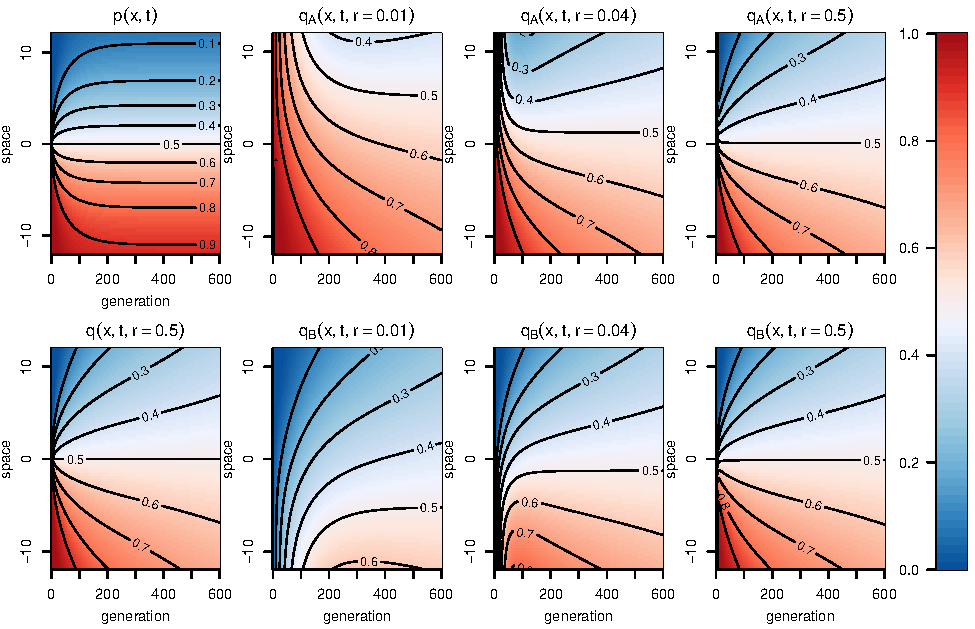
\includegraphics{figs/linked-frequencies-longtime.pdf}
    \caption{
        \textbf{Probabilities of $A$ ancestry,}
        across space (vertical axis, in units of $\sigma$) 
        and time (horizontal axis, in generations).
        In each plot, color corresponds to the expected frequency of $A$ ancestry
        at a particular location in time and space.
        The selection coefficient is $s=.02$.
        \textbf{Top left:} at the selected site, showing establishment and stabilization of the cline
        on a time scale of $1/s=50$ generations.
        \textbf{Bottom left:} at an unliked site,
        with cline flattening continuing with $\sqrt{t}$.
        Remaining figures show frequencies of $A$ ancestry \emph{conditional}
        on the ancestry at the selected site,
        at different distances from the selected site ($r=.01$, .04, and 0.5 Morgans),
        as described in the text (see definition of $q_z(x,t,r)$).
        See figure \ref{fig:linked_cline_heatmaps}
        for the same figure over a shorter period of time.
    }
    \label{sfig:linked_cline_heatmaps_longtime}
\end{figure}




\begin{figure}
    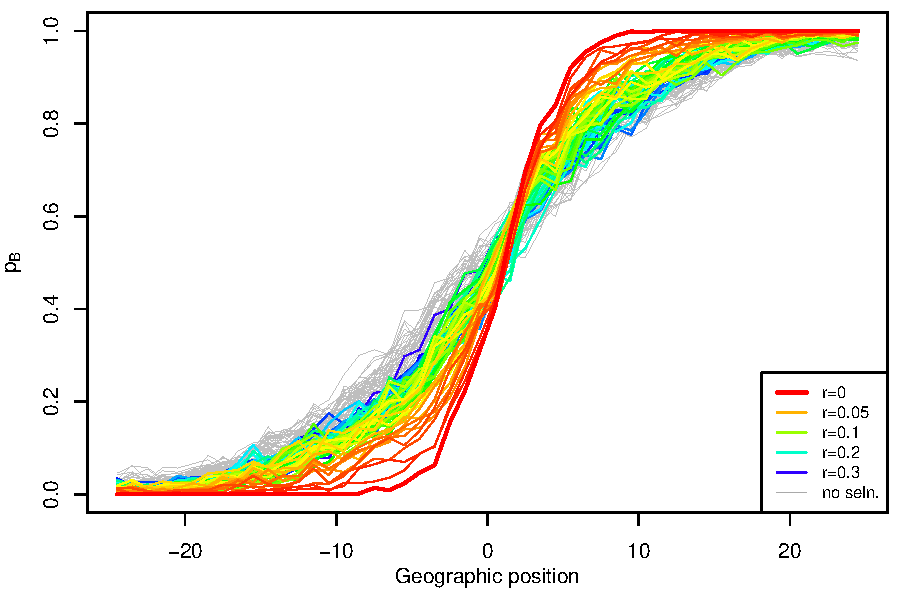
\includegraphics{{figs/alleleFrequencies_sim_s0.01_tau100_closely_linked}.pdf}
    \caption{
    Frequency of ancestry $B$,
    across geography at different physical positions on the genome, simulated for a hybrid zone
     $T=100$ generations after secondary contact, with $s=0.1$,
     using 50 demes, each with 500 diploid individuals and $\sigma=1$.
    Each line represents a locus some distance $r$ away from the true target of selection with colors corresponding to different values of $r$, transitioning from red (tight linkage to selected site) to blue (distantly linked).
    Grey lines represent the same positions from a simulation with
    identical parameters except that $s=0$. 
    Corresponding theoretical quantities are shown juxtaposed in Figure \ref{fig:alleleFreq_tau100_comparison};
    the same plot is shown with weaker selection in Figure \ref{alleleFreq_tau100_weaker_s} and at a longer time in Figure \ref{alleleFreq_tau1000}.
}\label{alleleFreq_tau100}
\end{figure}



\begin{figure}
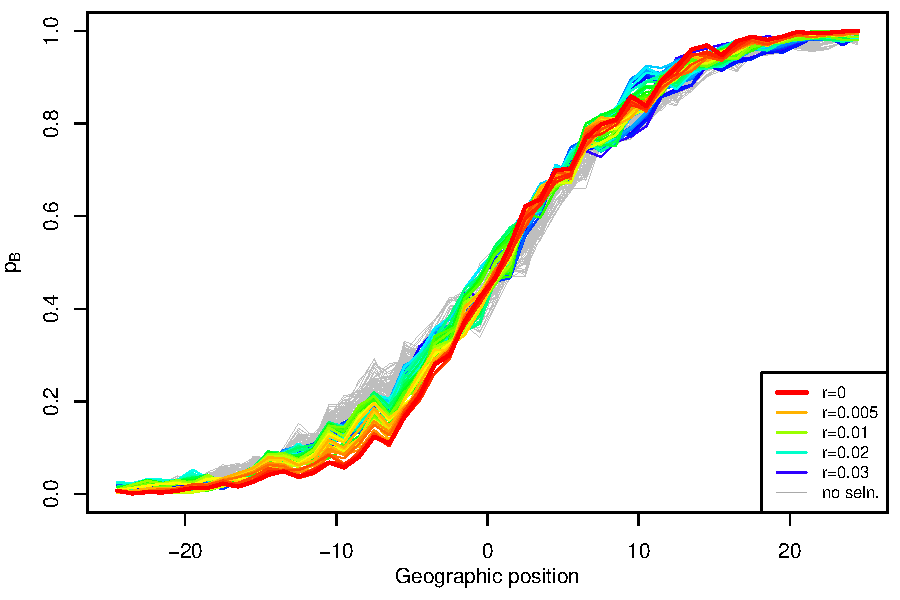
\includegraphics{figs/alleleFrequencies_sim_s01_tau100_closely_linked.pdf}
\caption{
    Frequency of ancestry $B$,
    across geography and at several physical positions on the genome, simulated for a hybrid zone
     $T=100$ generations after secondary contact,
    and with $s=0.01$.
    The simulated zone had 50 demes, each with a population size of 500 diploid individuals.
    Each line represents a locus some distance $r$ away from the true target of selection, 
    and $r=0$ represents the locus that is under selection. Grey lines represent the same positions from a simulation with
    identical parameters except that $s=0$.
}\label{alleleFreq_tau100_weaker_s}
\end{figure}

\begin{figure}
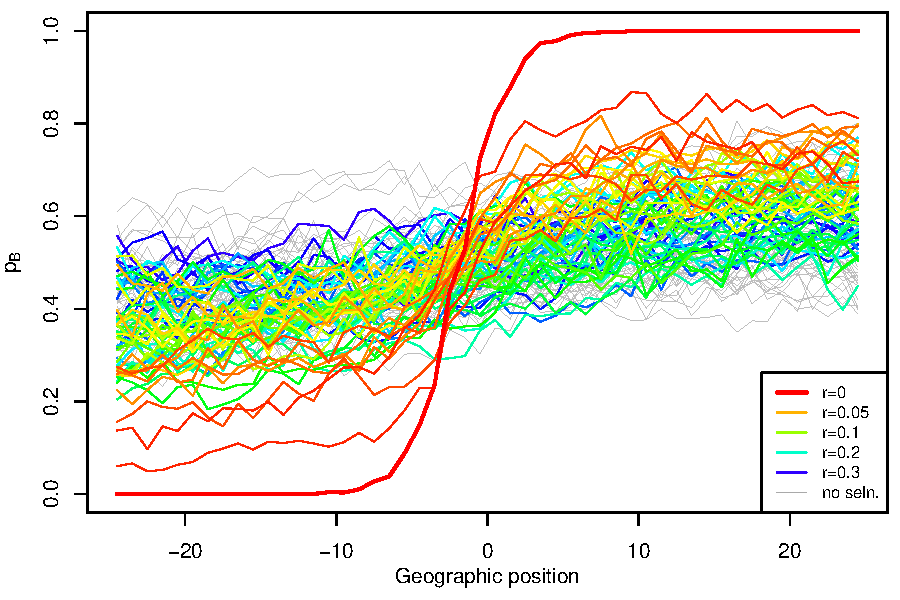
\includegraphics{figs/alleleFrequencies_sim_s1_tau1000.pdf}
\caption{
    Frequency of ancestry $B$,
    across geography and at several physical positions on the genome, simulated for a hybrid zone
     $T=1000$ generations after secondary contact,
    and with $s=0.1$.
    The simulated zone had 50 demes, each with a population size of 500 diploid individuals.
    Each line represents a locus some distance $r$ away from the true target of selection, 
    and $r=0$ represents the locus that is under selection. Grey lines represent the same positions from a simulation with
    identical parameters except that $s=0$.
 }\label{alleleFreq_tau1000}
\end{figure}

\begin{figure}
    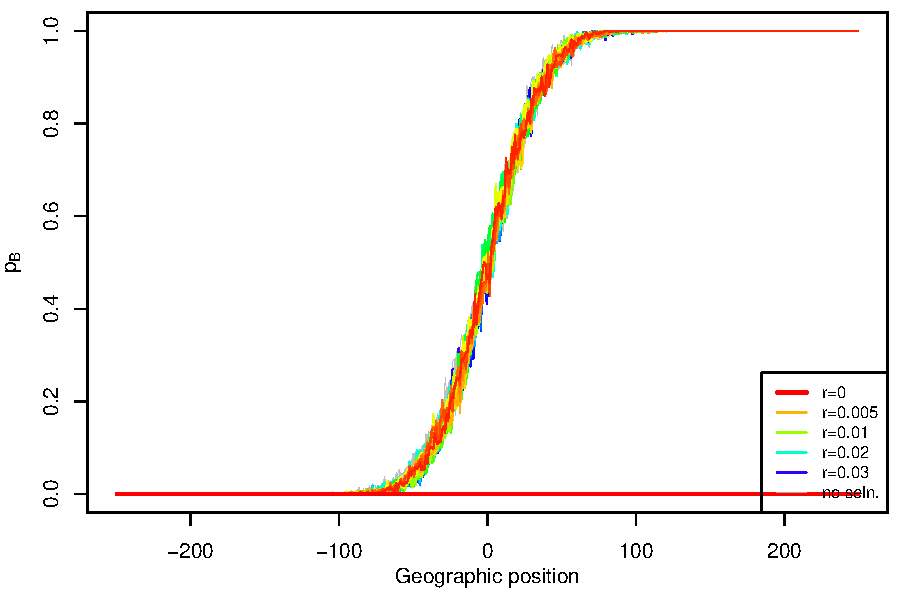
\includegraphics{{figs/alleleFrequencies_sim_SIGMA3_Ninds250000_ndemes500_s0.01_tau100}.pdf}
\caption{
    Frequency of ancestry $B$,
    across geography and at several physical positions on the genome, simulated for a hybrid zone
    $T=100$ generations after secondary contact,
    and with $s=0.01$.
    The simulated zone had 500 demes, each with a population size of 500 diploid individuals.
    Each line represents a locus some distance $r$ away from the true target of selection, 
    and $r=0$ represents the locus that is under selection. Grey lines represent the same positions from a simulation with
    identical parameters except that $s=0$.
}\label{sfig:extra_long_cline}
\end{figure}



\begin{figure}
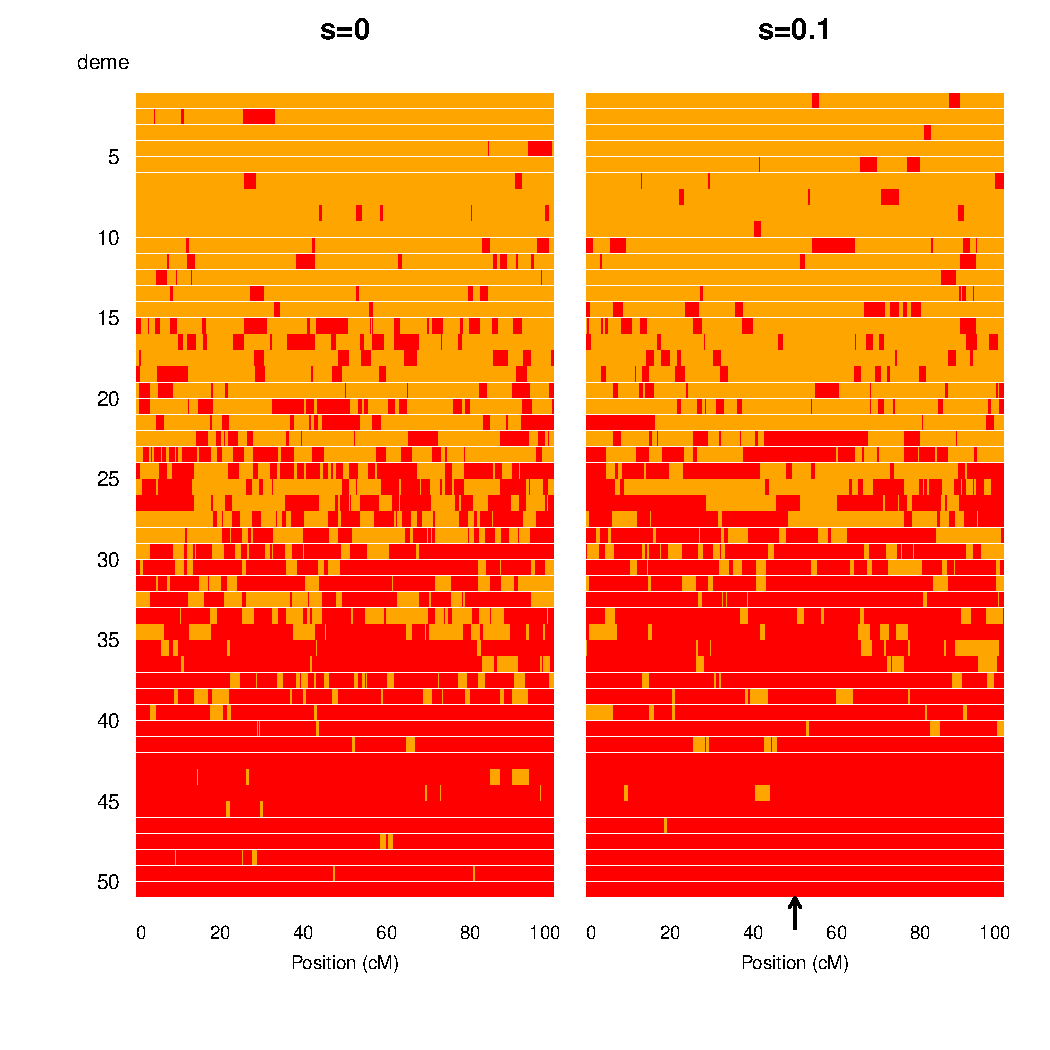
\includegraphics[width=\textwidth]{figs/plot_chromosomes_tau100.pdf}
\caption{Randomly sampled chromosomes  across a hybrid zone of age $T=100$. Here we compare chromosomes of length 1M from a neutral zone to one that has a single under-dominant locus ($s=0.1$) in the middle of the chromosome (indicated by black arrow). Red blocks along the chromosome denote ancestry $B$, and orange blocks are ancestry $A$.
 }\label{Fig:resistanceToIntrogression100g}
\end{figure}


\begin{figure}
    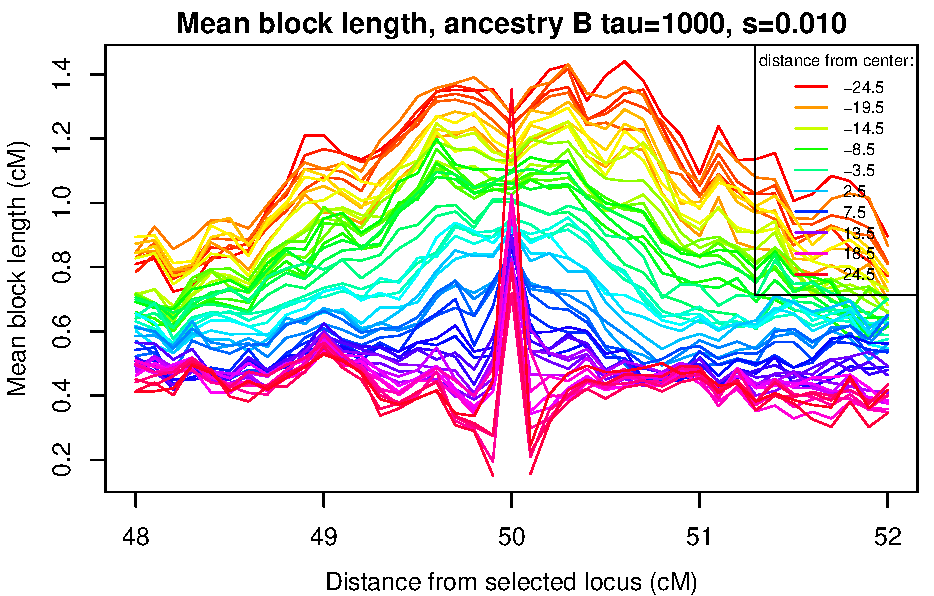
\includegraphics{{figs/simulation_SIGMA1_Ninds25000_ndemes50_s0.01_tau1000_blocksAlongChromAncBConditioning_nonnormalized}.pdf}
    \caption{
        \textbf{Mean haplotype lengths of $B$ haplotypes}, $l_B(x,m)$,
        across the genome (horizontal axis) and at different spatial locations (colored lines),
        from a simulation with 50 demes having 500 individuals each, $s=0.01$, $\sigma=1$, and after $T=1000$ generations.
    } \label{sfig:blocksAlongChromAncBConditioning_nonnormalized}
\end{figure}

\begin{figure}
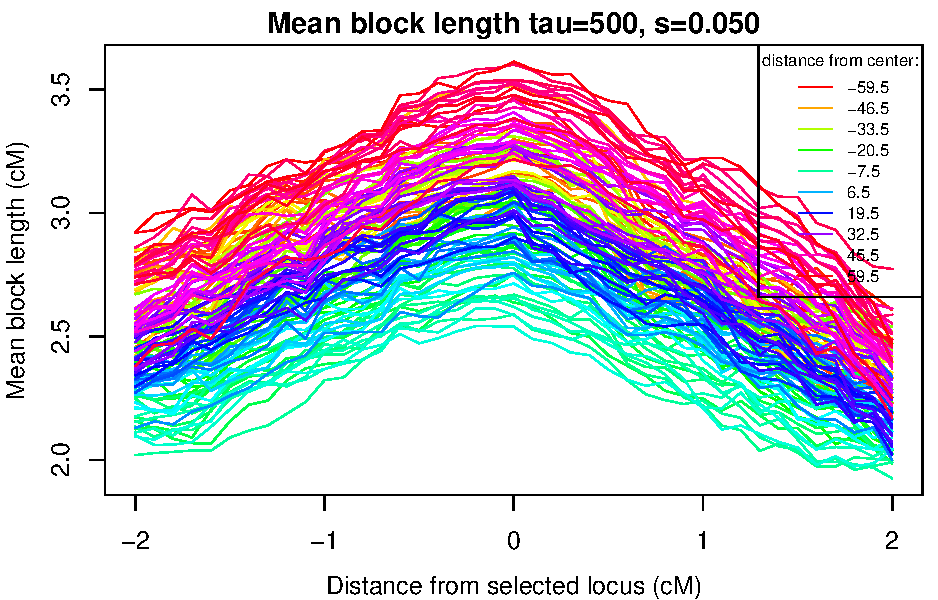
\includegraphics[width=\textwidth]{{figs/results_runid_753324_chr1_start0.48_stop0.52_by0.001_blocksAlongChromNoConditioning_nonnormalized}.pdf}
\caption{
    \textbf{Mean enclosing block length $l(m,x)$}, across the genome (horizontal axis)
    and at different geographic positions (different colored lines).
    Results are from a simulation with 120 demes of 200 diploids each, selection $s=.05$, dispersal $\sigma=3$, 
    and after $T=500$ generations.
}\label{Fig:meanBlockLengthsUnconditioned}
\end{figure}


\begin{figure}
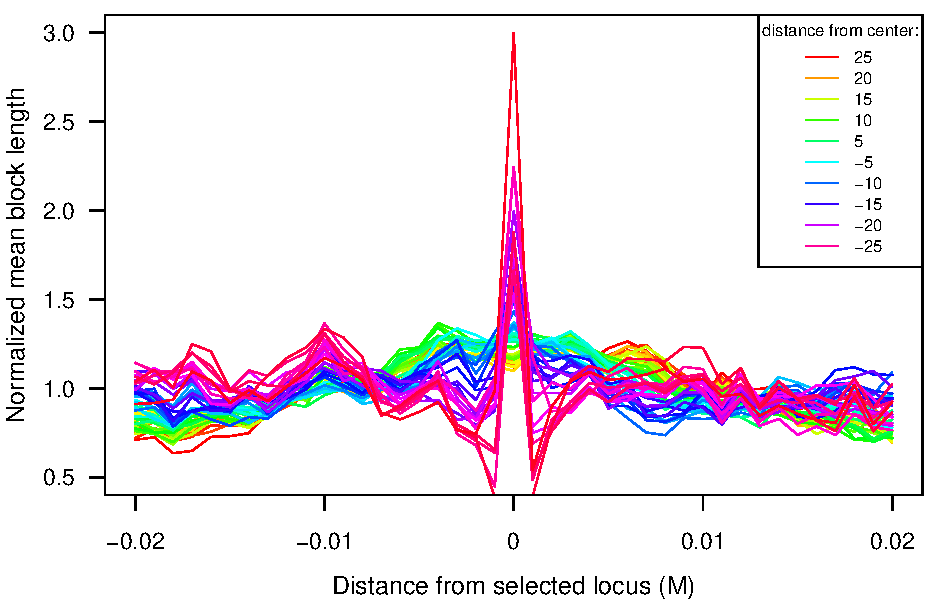
\includegraphics{figs/blocksAlongChromAncBConditioning.pdf}
\caption{
    \textbf{Normalized mean enclosing block length}, $\bar l_B(m,x)$, after $T=1000$ generations,
    against position relative to the selected locus (horizontal axis)
    located in the center of a 1M chromosome.
    Each line shows the mean block length at that spatial and genomic position
    divided by the mean over the chromosome at that location;
    the simulation was run with $s=0.01$ and $\sigma=1$,
    50 demes, each containing 500 diploid individuals.
}\label{Fig:blockLengths}
\end{figure}


\begin{figure}
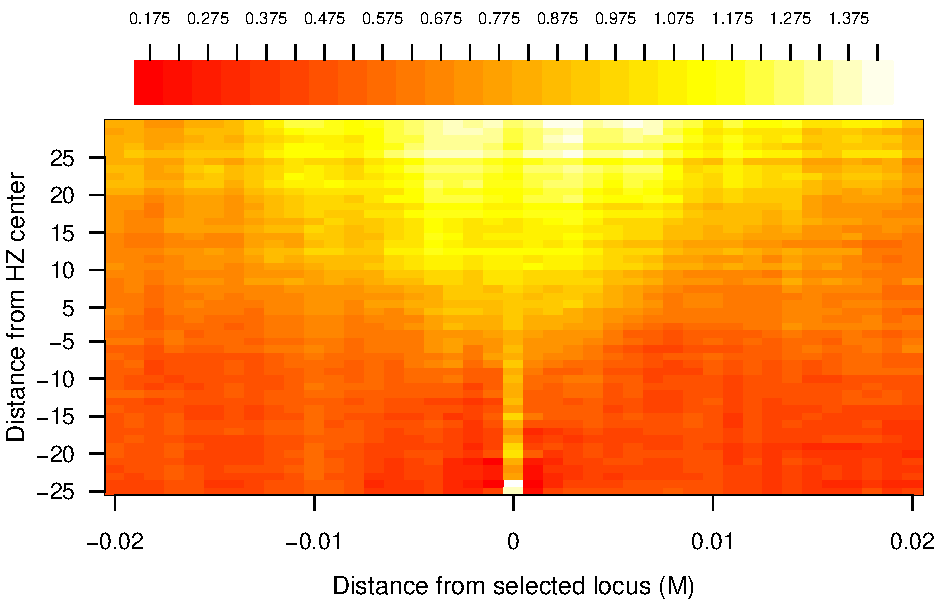
\includegraphics{figs/blocksAlongChromHeatmapAncBConditioning.pdf}
\caption{Heatmap of mean block length $l_B(m)$ along a simulated chromosome under $T=1000$, $s=0.01$ and $\sigma=1$,
    50 demes, each containing 500 diploid individuals. }\label{Supp:blockLengthHeatmap}
\end{figure}




\begin{figure}
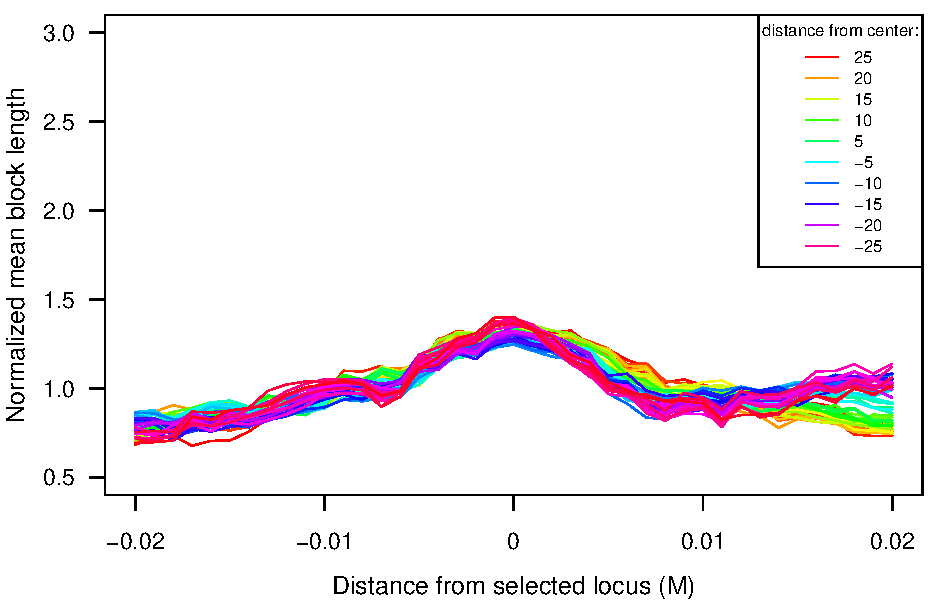
\includegraphics{figs/blocksAlongChromNoConditioning.pdf}
\caption{Mean block length $l(m)$, without conditioning on ancestry, surrounding a given position along the genome with a single underdominant site with parameters as for Fig~\ref{Fig:blockLengths}. ($s=0.01, T=1000, \sigma=1$). }\label{Supp:blockLengthNoAnc}
\end{figure}

\begin{figure}
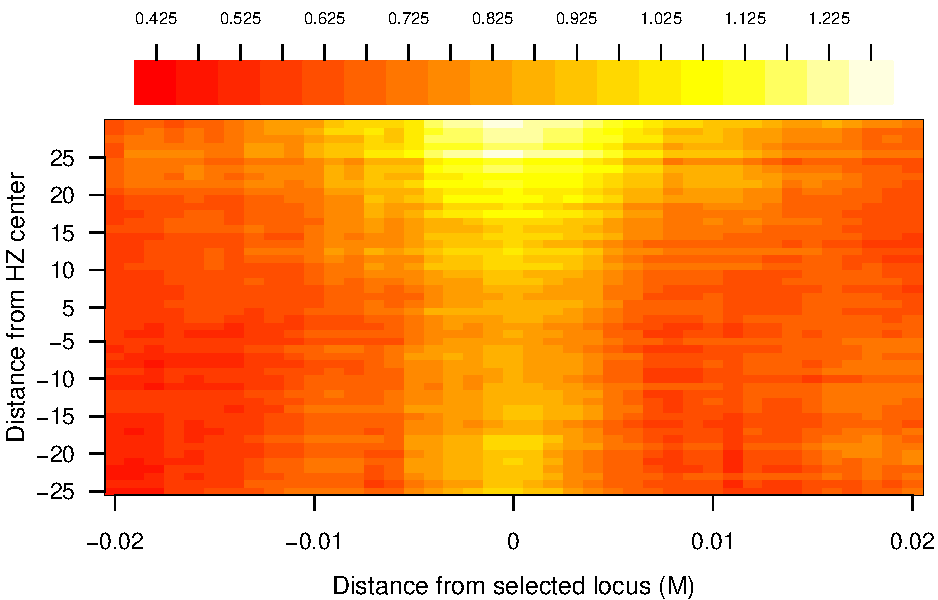
\includegraphics{figs/blocksAlongChromHeatmap.pdf}
\caption{Heatmap of mean block length $l(m)$, without conditioning on ancestry, along a simulated chromosome with a single underdominant site, with parameters as for Fig~\ref{Fig:blockLengths} ($s=0.01, T=1000, \sigma=1$) }\label{Supp:blockLengthHeatmapNoAnc}
\end{figure}


\begin{figure}
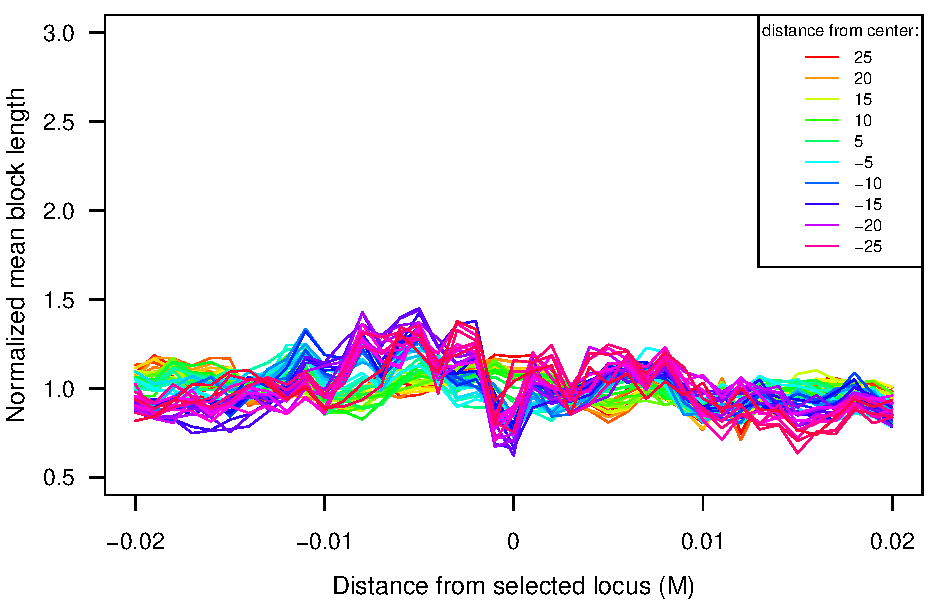
\includegraphics{figs/adjacentBlocksAlongChromAncBConditioning.pdf}
\caption{Mean block length of $l_A(m\pm)$ across chromosome with single under dominant site, conditioning on ancestry $B$ at the selected locus, with parameters as for Fig~\ref{Fig:blockLengths} ($s=0.01, T=1000, \sigma=1$)}\label{Supp:adjacentBlocks}
\end{figure}


\begin{figure}
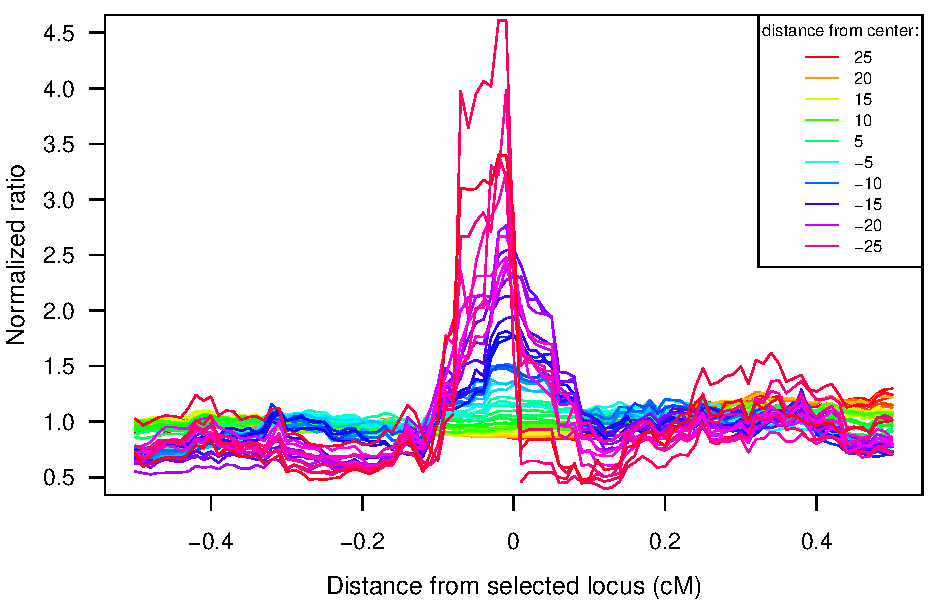
\includegraphics{figs/s0point01_ratioAdjacentBlocksAlongChromAncBConditioningHighRes.pdf}
    \caption{The normalized statistic $\bar C(m,x)$: the ratio $\frac{2\sum{l_B(m_i)}}{\sum{l_A(m_i-)+I_A(m_i+)}}$ of mean block length and mean adjacent block lengths across a simulated chromosome with a single underdominant site and conditioning on ancestry $B$ at the selected site ($s=0.01, T=1000$).  Each line represents a deme and is normalized by mean block length across the chromosome in the deme. This  simulation corresponds to that represented in Figure~\ref{Fig:blockLengthsZoom}; note the difference in y-axis scale.}\label{Supp:ratioBlockAdjacent}
\end{figure}


\begin{figure}
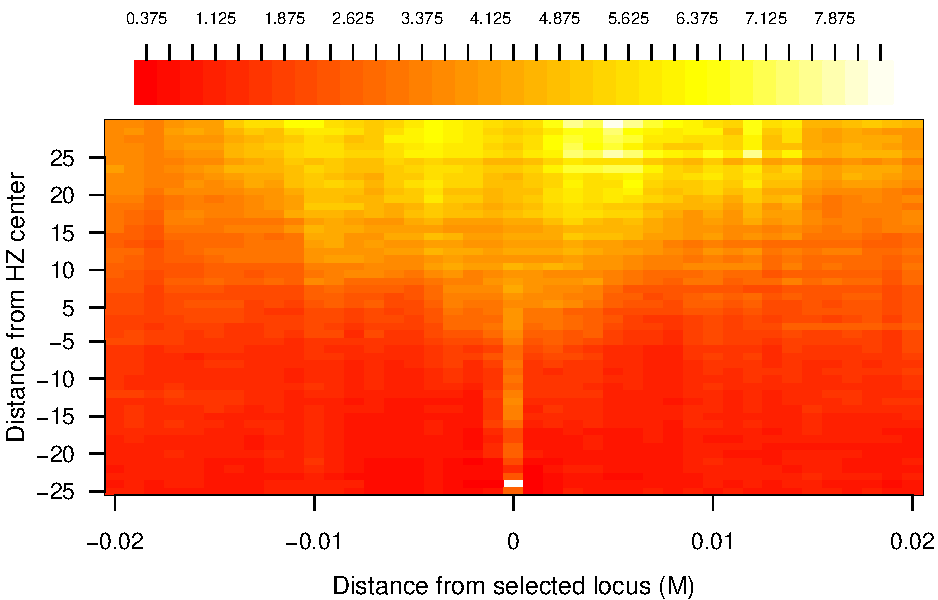
\includegraphics{figs/ratioAdjacentBlocksAlongChromHeatmapAncBConditioning.pdf}
    \caption{Heatmap of $C(m,x)=\frac{2\sum{l_B(m_i)}}{\sum{l_A(m_i-)+I_A(m_i+)}}$ across a simulated chromosome with a single underdominant site and conditioning on ancestry $B$ at the selected site and parameters as for Fig.~\ref{Fig:blockLengths} ($s=0.01, T=1000, \sigma=1$). }\label{Supp:ratioBlockAdjacentHeatmap}
\end{figure}


\begin{figure}
    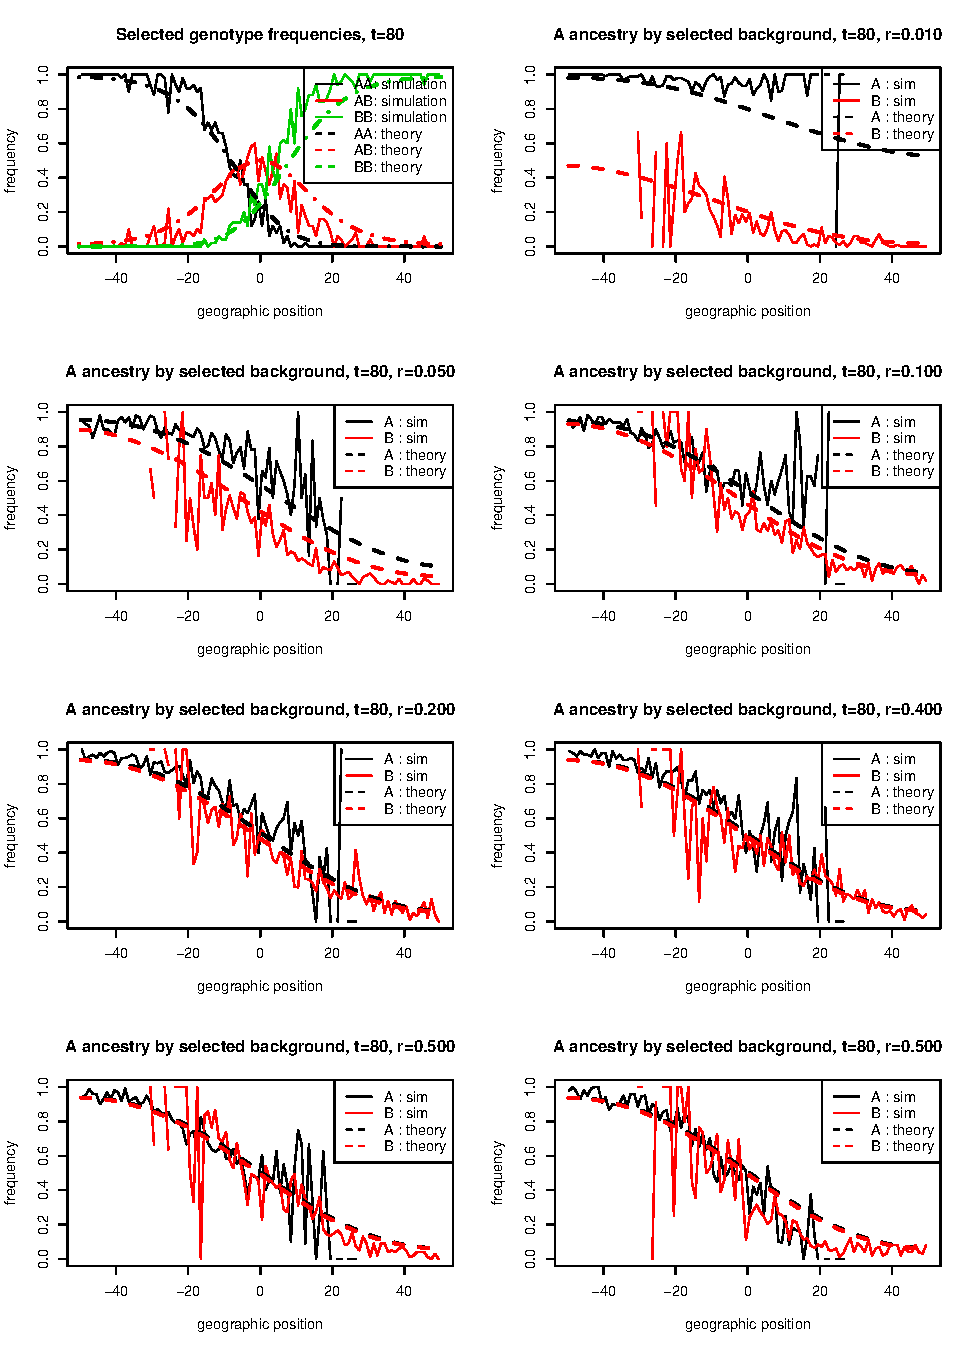
\includegraphics[height=0.8\textheight]{figs/cond_freqs_comparison_tau_80.pdf}
    \caption{
        \textbf{Conditional frequencies of ancestry $A$ at $\tau=80$},
        comparing simulation and theory, with $\sigma=3$ deme spacings, $s=0.05$, and 50 individuals per deme.
        The top left figure shows observed and expected genotype frequencies for the two homozygotes and the heterozygote at the selected locus;
        expected genotype counts were obtained assuming random mating,
        and by solving equation \eqref{eqn:cline_pde} numerically.
        The remaining figures show observed and expected frequencies of $A$ ancestry,
        separately conditioned on the identity of the linked allele at the selected site.
        Observed frequencies become much noisier where the linked allele becomes rarer.
    } \label{sfig:condAlleleFreq_tau80_comparison}
\end{figure}


\begin{figure}
    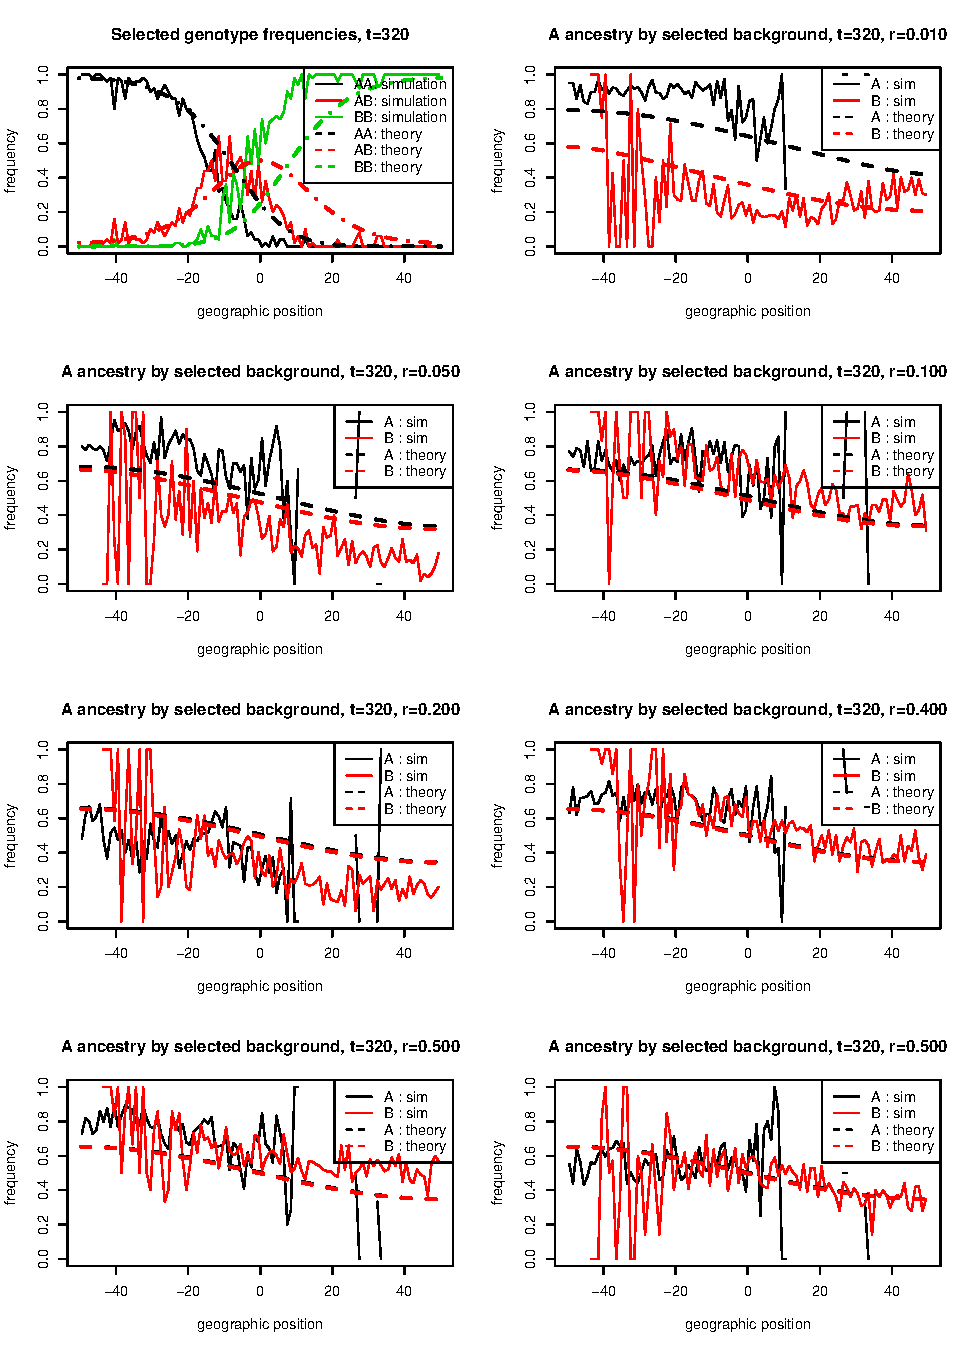
\includegraphics{figs/cond_freqs_comparison_tau_320.pdf}
    \caption{
        \textbf{Conditional frequencies of ancestry $A$ at $\tau=320$},
        as in figure \ref{sfig:condAlleleFreq_tau80_comparison}.
        Deviations are larger than at $\tau=80$, 
        due to genetic drift.
    } \label{sfig:condAlleleFreq_tau320_comparison}
\end{figure}


\begin{figure}
    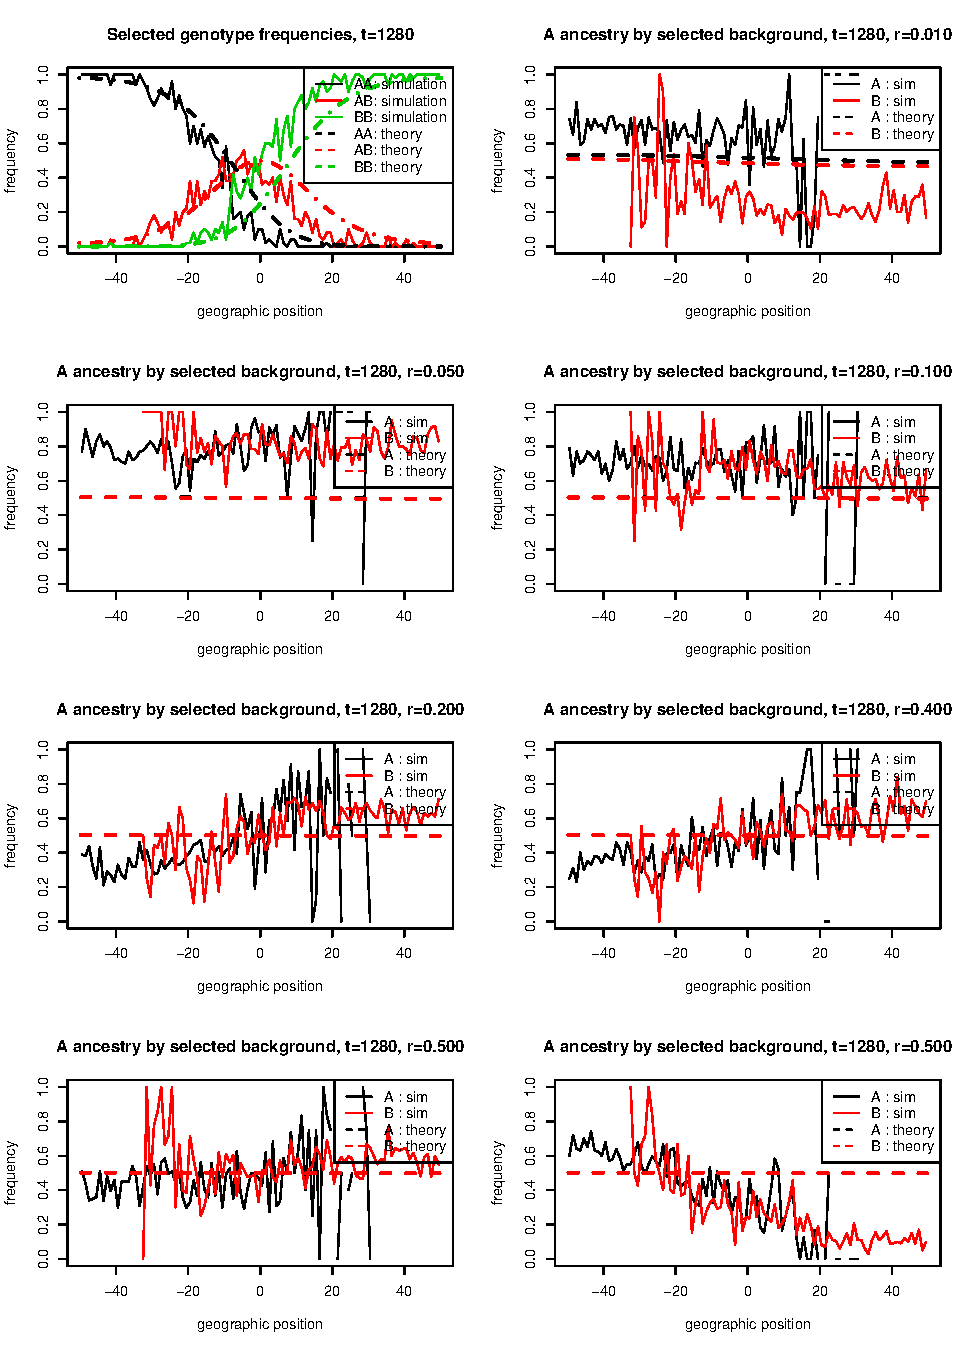
\includegraphics{figs/cond_freqs_comparison_tau_1280.pdf}
    \caption{
        \textbf{Conditional frequencies of ancestry $A$ at $\tau=1280$},
        as in figure \ref{sfig:condAlleleFreq_tau80_comparison}.
        Deviations are larger still than at $\tau=320$, 
        due to genetic drift.
    } \label{sfig:condAlleleFreq_tau1280_comparison}
\end{figure}
\clearpage
\begin{figure}
    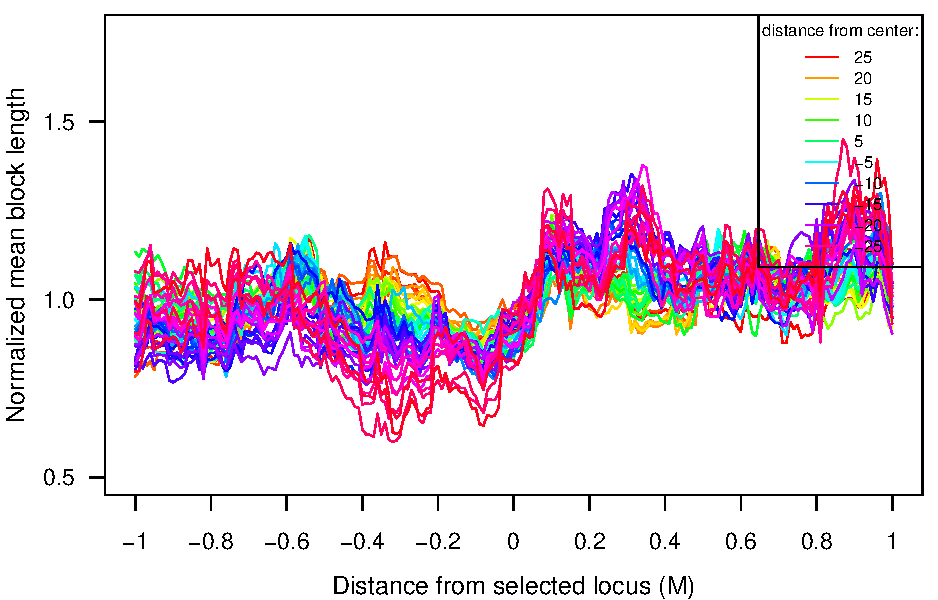
\includegraphics{figs/s001_adjacentBlocksAlongChromAncBConditioning}
    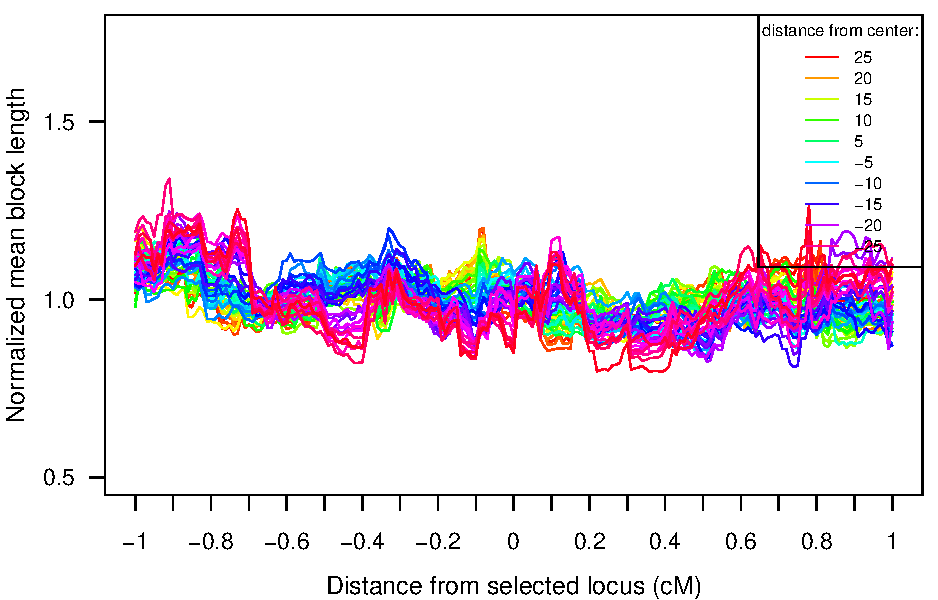
\includegraphics{figs/s001_adjacentBlocksAlongChromNoConditioningHighRes}
        \caption{
     Normalized ancestry $B$ block lengths (top) and all ancestry block lengths (bottom) along chromosome under $s=0.001$ and other parameters as for Fig.~\ref{Fig:blockLengths} ($\tau=1000,\sigma=1$). } \label{sfig:blockLengthPlot_t1000_s0.001}
\end{figure}


% \end{document}


\end{document}
